\documentclass[]{article}
\usepackage{fullpage,graphicx,psfrag,amsmath,amsfonts,verbatim}
\usepackage[small,bf]{caption}
\usepackage{hyperref,natbib}
\usepackage{longtable,booktabs}
\newcommand\tightlist{}

%\input defs.tex
\usepackage{titlesec}
\newcommand{\sectionbreak}{\clearpage}


%% Raw code highlight
\usepackage{color}
\usepackage{fancyvrb}
\newcommand{\VerbBar}{|}
\newcommand{\VERB}{\Verb[commandchars=\\\{\}]}
\DefineVerbatimEnvironment{Highlighting}{Verbatim}{commandchars=\\\{\}}
% Add ',fontsize=\small' for more characters per line
\usepackage{framed}
\definecolor{shadecolor}{RGB}{248,248,248}
\newenvironment{Shaded}{\begin{snugshade}}{\end{snugshade}}
\newcommand{\KeywordTok}[1]{\textcolor[rgb]{0.13,0.29,0.53}{\textbf{#1}}}
\newcommand{\DataTypeTok}[1]{\textcolor[rgb]{0.13,0.29,0.53}{#1}}
\newcommand{\DecValTok}[1]{\textcolor[rgb]{0.00,0.00,0.81}{#1}}
\newcommand{\BaseNTok}[1]{\textcolor[rgb]{0.00,0.00,0.81}{#1}}
\newcommand{\FloatTok}[1]{\textcolor[rgb]{0.00,0.00,0.81}{#1}}
\newcommand{\ConstantTok}[1]{\textcolor[rgb]{0.00,0.00,0.00}{#1}}
\newcommand{\CharTok}[1]{\textcolor[rgb]{0.31,0.60,0.02}{#1}}
\newcommand{\SpecialCharTok}[1]{\textcolor[rgb]{0.00,0.00,0.00}{#1}}
\newcommand{\StringTok}[1]{\textcolor[rgb]{0.31,0.60,0.02}{#1}}
\newcommand{\VerbatimStringTok}[1]{\textcolor[rgb]{0.31,0.60,0.02}{#1}}
\newcommand{\SpecialStringTok}[1]{\textcolor[rgb]{0.31,0.60,0.02}{#1}}
\newcommand{\ImportTok}[1]{#1}
\newcommand{\CommentTok}[1]{\textcolor[rgb]{0.56,0.35,0.01}{\textit{#1}}}
\newcommand{\DocumentationTok}[1]{\textcolor[rgb]{0.56,0.35,0.01}{\textbf{\textit{#1}}}}
\newcommand{\AnnotationTok}[1]{\textcolor[rgb]{0.56,0.35,0.01}{\textbf{\textit{#1}}}}
\newcommand{\CommentVarTok}[1]{\textcolor[rgb]{0.56,0.35,0.01}{\textbf{\textit{#1}}}}
\newcommand{\OtherTok}[1]{\textcolor[rgb]{0.56,0.35,0.01}{#1}}
\newcommand{\FunctionTok}[1]{\textcolor[rgb]{0.00,0.00,0.00}{#1}}
\newcommand{\VariableTok}[1]{\textcolor[rgb]{0.00,0.00,0.00}{#1}}
\newcommand{\ControlFlowTok}[1]{\textcolor[rgb]{0.13,0.29,0.53}{\textbf{#1}}}
\newcommand{\OperatorTok}[1]{\textcolor[rgb]{0.81,0.36,0.00}{\textbf{#1}}}
\newcommand{\BuiltInTok}[1]{#1}
\newcommand{\ExtensionTok}[1]{#1}
\newcommand{\PreprocessorTok}[1]{\textcolor[rgb]{0.56,0.35,0.01}{\textit{#1}}}
\newcommand{\AttributeTok}[1]{\textcolor[rgb]{0.77,0.63,0.00}{#1}}
\newcommand{\RegionMarkerTok}[1]{#1}
\newcommand{\InformationTok}[1]{\textcolor[rgb]{0.56,0.35,0.01}{\textbf{\textit{#1}}}}
\newcommand{\WarningTok}[1]{\textcolor[rgb]{0.56,0.35,0.01}{\textbf{\textit{#1}}}}
\newcommand{\AlertTok}[1]{\textcolor[rgb]{0.94,0.16,0.16}{#1}}
\newcommand{\ErrorTok}[1]{\textcolor[rgb]{0.64,0.00,0.00}{\textbf{#1}}}
\newcommand{\NormalTok}[1]{#1}
%% change fontsize of R code
\let\oldShaded\Shaded
\let\endoldShaded\endShaded
\renewenvironment{Shaded}{\footnotesize\oldShaded}{\endoldShaded}


\title{Notebook: Races vs Tournament}
\date{Last updated: 09 June, 2017}


\begin{document}
\maketitle


%\newpage
\tableofcontents
\newpage

\section{Descriptive statistics}\label{descriptive-statistics}

The Table below shows summary statistics for the main variables in our
sample. It also provides p-values from Kruskal-Wallis non-parametric
test, showing no evidence of systematic differences across the three
treatment groups (the lowest p-value was xxxx). Hence, our randomization
appears successful.

\begin{Shaded}
\begin{Highlighting}[]
\CommentTok{# Library}
\KeywordTok{require}\NormalTok{(xtable)}
\KeywordTok{require}\NormalTok{(races)}

\CommentTok{# Load data}
\KeywordTok{data}\NormalTok{(races)}
\KeywordTok{attach}\NormalTok{(races)}

\CommentTok{# Define help functions}
\NormalTok{balance.test <-}\StringTok{ }\ControlFlowTok{function}\NormalTok{(x) \{}
\NormalTok{    l <-}\StringTok{ }\KeywordTok{split}\NormalTok{(x, treatment)}
    \KeywordTok{kruskal.test}\NormalTok{(l)}\OperatorTok{$}\NormalTok{p.val}
\NormalTok{\}}
\NormalTok{nomiss <-}\StringTok{ }\ControlFlowTok{function}\NormalTok{(x) }\KeywordTok{sum}\NormalTok{(}\OperatorTok{!}\KeywordTok{is.na}\NormalTok{(x))}

\CommentTok{# New variables}
\NormalTok{year <-}\StringTok{ }\KeywordTok{as.numeric}\NormalTok{(}\KeywordTok{format}\NormalTok{(member_date, }\StringTok{"%Y"}\NormalTok{))}
\NormalTok{month <-}\StringTok{ }\KeywordTok{as.numeric}\NormalTok{(}\KeywordTok{format}\NormalTok{(member_date, }\StringTok{"%m"}\NormalTok{))}
\NormalTok{hours <-}\StringTok{ }\NormalTok{week1 }\OperatorTok{+}\StringTok{ }\NormalTok{week2 }\OperatorTok{+}\StringTok{ }\NormalTok{week3 }\OperatorTok{+}\StringTok{ }\NormalTok{week4}
\NormalTok{rating <-}\StringTok{ }\NormalTok{mm_rating}
\NormalTok{submissions <-}\StringTok{ }\NormalTok{mm_events}
\NormalTok{registrations <-}\StringTok{ }\NormalTok{mm_reg}
\NormalTok{lpaid <-}\StringTok{ }\KeywordTok{log}\NormalTok{(paid)}

\CommentTok{# Dataset}
\NormalTok{dat <-}\StringTok{ }\KeywordTok{data.frame}\NormalTok{(year, month, rating, submissions, registrations, }
\NormalTok{    lpaid, nwins, ntop10, risk, hours, timezone)}

\CommentTok{# Compute summary statistics}
\NormalTok{mu <-}\StringTok{ }\KeywordTok{sapply}\NormalTok{(dat, mean, }\DataTypeTok{na.rm =} \OtherTok{TRUE}\NormalTok{)}
\NormalTok{q50 <-}\StringTok{ }\KeywordTok{sapply}\NormalTok{(dat, median, }\DataTypeTok{na.rm =} \OtherTok{TRUE}\NormalTok{)}
\NormalTok{std <-}\StringTok{ }\KeywordTok{sapply}\NormalTok{(dat, sd, }\DataTypeTok{na.rm =} \OtherTok{TRUE}\NormalTok{)}
\NormalTok{pval <-}\StringTok{ }\KeywordTok{sapply}\NormalTok{(dat, balance.test)}
\NormalTok{n <-}\StringTok{ }\KeywordTok{sapply}\NormalTok{(dat, nomiss)}

\CommentTok{# Render table}
\NormalTok{tab <-}\StringTok{ }\KeywordTok{cbind}\NormalTok{(mu, q50, std, n, pval)}
\KeywordTok{colnames}\NormalTok{(tab) <-}\StringTok{ }\KeywordTok{c}\NormalTok{(}\StringTok{"Mean"}\NormalTok{, }\StringTok{"Median"}\NormalTok{, }\StringTok{"St.Dev."}\NormalTok{, }\StringTok{"Obs."}\NormalTok{, }\StringTok{"P-value"}\NormalTok{)}
\NormalTok{xtab <-}\StringTok{ }\KeywordTok{xtable}\NormalTok{(tab)}
\KeywordTok{digits}\NormalTok{(xtab) <-}\StringTok{ }\KeywordTok{c}\NormalTok{(}\KeywordTok{rep}\NormalTok{(}\DecValTok{0}\NormalTok{, }\KeywordTok{ncol}\NormalTok{(tab)), }\DecValTok{3}\NormalTok{)}
\KeywordTok{align}\NormalTok{(xtab) <-}\StringTok{ }\KeywordTok{c}\NormalTok{(}\StringTok{"@\{\}l"}\NormalTok{, }\KeywordTok{rep}\NormalTok{(}\StringTok{"r"}\NormalTok{, }\KeywordTok{ncol}\NormalTok{(tab)))}
\KeywordTok{caption}\NormalTok{(xtab) <-}\StringTok{ "Summary statistics"}
\KeywordTok{label}\NormalTok{(xtab) <-}\StringTok{ "summary"}

\KeywordTok{detach}\NormalTok{(races)}
\end{Highlighting}
\end{Shaded}

\begin{Shaded}
\begin{Highlighting}[]
\KeywordTok{render.xtable}\NormalTok{(xtab)}
\end{Highlighting}
\end{Shaded}

\begin{table}
\centering
\caption{Summary statistics}
\label{summary}
\begin{tabular}{@{}lrrrrr}
  \\[-1.8ex]\hline\hline\\[-1.8ex]
 & Mean & Median & St.Dev. & Obs. & P-value \\ 
  \hline\\[-1.86ex]
year & 2010 & 2010 & 4 & 299 & 0.596 \\ 
  month & 6 & 6 & 4 & 299 & 0.793 \\ 
  rating & 1322 & 1278 & 425 & 205 & 0.989 \\ 
  submissions & 7 & 2 & 12 & 299 & 0.867 \\ 
  registrations & 18 & 9 & 23 & 299 & 0.626 \\ 
  lpaid & 8 & 8 & 3 & 139 & 0.791 \\ 
  nwins & 0 & 0 & 2 & 299 & 0.370 \\ 
  ntop10 & 2 & 0 & 5 & 299 & 0.273 \\ 
  risk & 6 & 7 & 2 & 279 & 0.958 \\ 
  hours & 31 & 24 & 25 & 277 & 0.995 \\ 
  timezone & 2 & 2 & 5 & 277 & 0.389 \\ 
   \hline\\[-1.8ex]
\end{tabular}
\end{table}

\section{Analysis of entry decision}\label{analysis-of-entry-decision}

We test differences in participation rates across treatment groups and
we find no significant differences using a Fisher's exact test. We
further test differences in participation rates between large and small
rooms. But we find no significant differences.

\begin{Shaded}
\begin{Highlighting}[]
\KeywordTok{data}\NormalTok{(races)}

\CommentTok{# Odds between treatments}
\NormalTok{tab <-}\StringTok{ }\KeywordTok{with}\NormalTok{(races, }\KeywordTok{table}\NormalTok{(submit, treatment))}
\KeywordTok{rownames}\NormalTok{(tab) <-}\StringTok{ }\KeywordTok{c}\NormalTok{(}\StringTok{"Not participating"}\NormalTok{, }\StringTok{"Participating"}\NormalTok{)}
\KeywordTok{print}\NormalTok{(tab)}
\end{Highlighting}
\end{Shaded}

\begin{verbatim}
##                    treatment
## submit              race tournament reserve
##   Not participating   73         67      73
##   Participating       26         33      27
\end{verbatim}

\begin{Shaded}
\begin{Highlighting}[]
\KeywordTok{fisher.test}\NormalTok{(tab)}
\end{Highlighting}
\end{Shaded}

\begin{verbatim}
## 
##  Fisher's Exact Test for Count Data
## 
## data:  tab
## p-value = 0.5255
## alternative hypothesis: two.sided
\end{verbatim}

\begin{Shaded}
\begin{Highlighting}[]
\CommentTok{# Odds between large & small rooms}
\NormalTok{tab.size <-}\StringTok{ }\KeywordTok{with}\NormalTok{(races, }\KeywordTok{table}\NormalTok{(submit, room_size))}
\KeywordTok{print}\NormalTok{(tab.size)}
\end{Highlighting}
\end{Shaded}

\begin{verbatim}
##        room_size
## submit  Large Small
##   FALSE   128    85
##   TRUE     52    34
\end{verbatim}

\begin{Shaded}
\begin{Highlighting}[]
\KeywordTok{fisher.test}\NormalTok{(tab.size)}
\end{Highlighting}
\end{Shaded}

\begin{verbatim}
## 
##  Fisher's Exact Test for Count Data
## 
## data:  tab.size
## p-value = 1
## alternative hypothesis: true odds ratio is not equal to 1
## 95 percent confidence interval:
##  0.5689643 1.6912635
## sample estimates:
## odds ratio 
##  0.9846648
\end{verbatim}

For each individual we observe a variable \(Z_i\), an indicator for the
assigned ``competition style'' of the room person \(i\) was competing
in; a binary outcome variable \(Y_i\), equal to 1 if person \(i\) made a
valid code submission during the competition {[}non example and with
score greater than zero{]}, and 0 otherwise; and a vector of covariates
\(X_i\), that include a skill rating and other measures of experience
and ability on the platform.

Since participation was a binary indicator, we estimate the logistic
regression model:

\[
    \Pr( Y_i = 1 \mid Z_i, X_i) = \lambda(\beta_0 + \beta_1 Z_i + X_i^\prime \gamma)
\]

where \(\lambda(\cdot)\) is the inverse of the logistic distribution
(the link function). {[}Results are below{]}

\begin{Shaded}
\begin{Highlighting}[]
\CommentTok{# New variables}
\KeywordTok{attach}\NormalTok{(races)}
\NormalTok{year <-}\StringTok{ }\KeywordTok{as.numeric}\NormalTok{(}\KeywordTok{format}\NormalTok{(member_date, }\StringTok{"%Y"}\NormalTok{))}
\NormalTok{month <-}\StringTok{ }\KeywordTok{as.numeric}\NormalTok{(}\KeywordTok{format}\NormalTok{(member_date, }\StringTok{"%m"}\NormalTok{))}
\NormalTok{hours <-}\StringTok{ }\NormalTok{week1 }\OperatorTok{+}\StringTok{ }\NormalTok{week2 }\OperatorTok{+}\StringTok{ }\NormalTok{week3 }\OperatorTok{+}\StringTok{ }\NormalTok{week4}
\NormalTok{rating <-}\StringTok{ }\NormalTok{(mm_rating }\OperatorTok{-}\StringTok{ }\KeywordTok{median}\NormalTok{(mm_rating, }\DataTypeTok{na.rm =} \OtherTok{TRUE}\NormalTok{))}\OperatorTok{/}\DecValTok{100}

\CommentTok{# Impute missing values}
\KeywordTok{set.seed}\NormalTok{(}\DecValTok{25978}\NormalTok{)}
\NormalTok{hours.imp <-}\StringTok{ }\KeywordTok{impute}\NormalTok{(hours, }\StringTok{"random"}\NormalTok{)}
\NormalTok{lhours.imp <-}\StringTok{ }\KeywordTok{log}\NormalTok{(hours.imp)}
\NormalTok{risk.imp <-}\StringTok{ }\KeywordTok{impute}\NormalTok{(risk, }\StringTok{"random"}\NormalTok{)}
\NormalTok{timezone.imp <-}\StringTok{ }\KeywordTok{impute}\NormalTok{(timezone, }\StringTok{"random"}\NormalTok{)}

\CommentTok{# New dataset}
\NormalTok{dat <-}\StringTok{ }\KeywordTok{data.frame}\NormalTok{(submit, treatment, rating, nwins, ntop10, year, }
\NormalTok{    month, lhours.imp, risk.imp, timezone.imp)}
\KeywordTok{detach}\NormalTok{(races)}

\CommentTok{# First model has no covariates (i.e., $\textbackslash{}gamma=0$)}
\KeywordTok{summary}\NormalTok{(m0 <-}\StringTok{ }\KeywordTok{glm}\NormalTok{(submit }\OperatorTok{~}\StringTok{ }\NormalTok{treatment, }\KeywordTok{binomial}\NormalTok{(logit), }\DataTypeTok{data =}\NormalTok{ dat))}
\end{Highlighting}
\end{Shaded}

\begin{verbatim}
## 
## Call:
## glm(formula = submit ~ treatment, family = binomial(logit), data = dat)
## 
## Deviance Residuals: 
##     Min       1Q   Median       3Q      Max  
## -0.8950  -0.7934  -0.7806   1.4891   1.6353  
## 
## Coefficients:
##                     Estimate Std. Error z value Pr(>|z|)    
## (Intercept)         -1.03236    0.22839  -4.520 6.18e-06 ***
## treatmenttournament  0.32418    0.31207   1.039    0.299    
## treatmentreserve     0.03774    0.32077   0.118    0.906    
## ---
## Signif. codes:  0 '***' 0.001 '**' 0.01 '*' 0.05 '.' 0.1 ' ' 1
## 
## (Dispersion parameter for binomial family taken to be 1)
## 
##     Null deviance: 358.81  on 298  degrees of freedom
## Residual deviance: 357.49  on 296  degrees of freedom
## AIC: 363.49
## 
## Number of Fisher Scoring iterations: 4
\end{verbatim}

\begin{Shaded}
\begin{Highlighting}[]
\CommentTok{# Whereas the second model adds the main skill rating measure}
\CommentTok{# (which is available only for xxx people) Rating is centered}
\CommentTok{# on the median}
\KeywordTok{summary}\NormalTok{(m1 <-}\StringTok{ }\KeywordTok{update}\NormalTok{(m0, }\StringTok{" ~ . + rating"}\NormalTok{))}
\end{Highlighting}
\end{Shaded}

\begin{verbatim}
## 
## Call:
## glm(formula = submit ~ treatment + rating, family = binomial(logit), 
##     data = dat)
## 
## Deviance Residuals: 
##     Min       1Q   Median       3Q      Max  
## -1.5846  -0.9441  -0.7840   1.2855   1.8284  
## 
## Coefficients:
##                     Estimate Std. Error z value Pr(>|z|)   
## (Intercept)         -0.81426    0.26711  -3.048  0.00230 **
## treatmenttournament  0.31570    0.36635   0.862  0.38882   
## treatmentreserve     0.20445    0.36931   0.554  0.57986   
## rating               0.10470    0.03597   2.911  0.00361 **
## ---
## Signif. codes:  0 '***' 0.001 '**' 0.01 '*' 0.05 '.' 0.1 ' ' 1
## 
## (Dispersion parameter for binomial family taken to be 1)
## 
##     Null deviance: 268.13  on 204  degrees of freedom
## Residual deviance: 258.38  on 201  degrees of freedom
##   (94 observations deleted due to missingness)
## AIC: 266.38
## 
## Number of Fisher Scoring iterations: 4
\end{verbatim}

\begin{Shaded}
\begin{Highlighting}[]
\CommentTok{# The third column adds other (complete) measures of skill}
\KeywordTok{summary}\NormalTok{(m2 <-}\StringTok{ }\KeywordTok{update}\NormalTok{(m0, }\StringTok{" ~ . + ntop10"}\NormalTok{))}
\end{Highlighting}
\end{Shaded}

\begin{verbatim}
## 
## Call:
## glm(formula = submit ~ treatment + ntop10, family = binomial(logit), 
##     data = dat)
## 
## Deviance Residuals: 
##     Min       1Q   Median       3Q      Max  
## -2.0105  -0.8662  -0.7528   1.4514   1.6920  
## 
## Coefficients:
##                     Estimate Std. Error z value Pr(>|z|)    
## (Intercept)         -1.15835    0.23813  -4.864 1.15e-06 ***
## treatmenttournament  0.37467    0.31631   1.185   0.2362    
## treatmentreserve     0.04241    0.32598   0.130   0.8965    
## ntop10               0.06511    0.03106   2.096   0.0361 *  
## ---
## Signif. codes:  0 '***' 0.001 '**' 0.01 '*' 0.05 '.' 0.1 ' ' 1
## 
## (Dispersion parameter for binomial family taken to be 1)
## 
##     Null deviance: 358.81  on 298  degrees of freedom
## Residual deviance: 350.99  on 295  degrees of freedom
## AIC: 358.99
## 
## Number of Fisher Scoring iterations: 4
\end{verbatim}

\begin{Shaded}
\begin{Highlighting}[]
\CommentTok{# Add time availability (hours), timezone , risk aversion}
\KeywordTok{summary}\NormalTok{(m3 <-}\StringTok{ }\KeywordTok{update}\NormalTok{(m0, }\StringTok{" ~ . + exp(lhours.imp) + timezone.imp"}\NormalTok{))}
\end{Highlighting}
\end{Shaded}

\begin{verbatim}
## 
## Call:
## glm(formula = submit ~ treatment + exp(lhours.imp) + timezone.imp, 
##     family = binomial(logit), data = dat)
## 
## Deviance Residuals: 
##     Min       1Q   Median       3Q      Max  
## -1.1727  -0.8213  -0.7498   1.4083   1.7619  
## 
## Coefficients:
##                      Estimate Std. Error z value Pr(>|z|)    
## (Intercept)         -1.409755   0.283258  -4.977 6.46e-07 ***
## treatmenttournament  0.297135   0.316698   0.938   0.3481    
## treatmentreserve     0.061330   0.324321   0.189   0.8500    
## exp(lhours.imp)      0.011430   0.004766   2.398   0.0165 *  
## timezone.imp         0.004223   0.025739   0.164   0.8697    
## ---
## Signif. codes:  0 '***' 0.001 '**' 0.01 '*' 0.05 '.' 0.1 ' ' 1
## 
## (Dispersion parameter for binomial family taken to be 1)
## 
##     Null deviance: 358.81  on 298  degrees of freedom
## Residual deviance: 351.39  on 294  degrees of freedom
## AIC: 361.39
## 
## Number of Fisher Scoring iterations: 4
\end{verbatim}

\begin{Shaded}
\begin{Highlighting}[]
\CommentTok{# Add skills and time}
\KeywordTok{summary}\NormalTok{(m4 <-}\StringTok{ }\KeywordTok{update}\NormalTok{(m1, }\StringTok{" ~ . + exp(lhours.imp) + timezone.imp"}\NormalTok{))}
\end{Highlighting}
\end{Shaded}

\begin{verbatim}
## 
## Call:
## glm(formula = submit ~ treatment + rating + exp(lhours.imp) + 
##     timezone.imp, family = binomial(logit), data = dat)
## 
## Deviance Residuals: 
##     Min       1Q   Median       3Q      Max  
## -1.6719  -0.9375  -0.7294   1.2832   1.8461  
## 
## Coefficients:
##                      Estimate Std. Error z value Pr(>|z|)    
## (Intercept)         -1.247266   0.340366  -3.664 0.000248 ***
## treatmenttournament  0.266400   0.374072   0.712 0.476365    
## treatmentreserve     0.229904   0.373621   0.615 0.538330    
## rating               0.111473   0.036756   3.033 0.002423 ** 
## exp(lhours.imp)      0.014895   0.006628   2.247 0.024615 *  
## timezone.imp        -0.011784   0.030269  -0.389 0.697054    
## ---
## Signif. codes:  0 '***' 0.001 '**' 0.01 '*' 0.05 '.' 0.1 ' ' 1
## 
## (Dispersion parameter for binomial family taken to be 1)
## 
##     Null deviance: 268.13  on 204  degrees of freedom
## Residual deviance: 252.39  on 199  degrees of freedom
##   (94 observations deleted due to missingness)
## AIC: 264.39
## 
## Number of Fisher Scoring iterations: 4
\end{verbatim}

\begin{Shaded}
\begin{Highlighting}[]
\KeywordTok{summary}\NormalTok{(m5 <-}\StringTok{ }\KeywordTok{update}\NormalTok{(m2, }\StringTok{" ~ . + exp(lhours.imp) + timezone.imp"}\NormalTok{))}
\end{Highlighting}
\end{Shaded}

\begin{verbatim}
## 
## Call:
## glm(formula = submit ~ treatment + ntop10 + exp(lhours.imp) + 
##     timezone.imp, family = binomial(logit), data = dat)
## 
## Deviance Residuals: 
##     Min       1Q   Median       3Q      Max  
## -2.0727  -0.7995  -0.7167   1.2720   1.8193  
## 
## Coefficients:
##                      Estimate Std. Error z value Pr(>|z|)    
## (Intercept)         -1.581602   0.296419  -5.336 9.52e-08 ***
## treatmenttournament  0.347896   0.321877   1.081  0.27977    
## treatmentreserve     0.076423   0.329957   0.232  0.81684    
## ntop10               0.071545   0.032061   2.232  0.02565 *  
## exp(lhours.imp)      0.012696   0.004864   2.610  0.00905 ** 
## timezone.imp        -0.000406   0.026147  -0.016  0.98761    
## ---
## Signif. codes:  0 '***' 0.001 '**' 0.01 '*' 0.05 '.' 0.1 ' ' 1
## 
## (Dispersion parameter for binomial family taken to be 1)
## 
##     Null deviance: 358.81  on 298  degrees of freedom
## Residual deviance: 343.74  on 293  degrees of freedom
## AIC: 355.74
## 
## Number of Fisher Scoring iterations: 4
\end{verbatim}

\begin{Shaded}
\begin{Highlighting}[]
\CommentTok{# Compare models}
\NormalTok{models <-}\StringTok{ }\KeywordTok{list}\NormalTok{(m0, m1, m2, m3, m4, m5)}
\KeywordTok{stargazer}\NormalTok{(models, }\DataTypeTok{type =} \StringTok{"text"}\NormalTok{, }\DataTypeTok{keep.stat =} \KeywordTok{c}\NormalTok{(}\StringTok{"n"}\NormalTok{, }\StringTok{"ll"}\NormalTok{))}
\end{Highlighting}
\end{Shaded}

\begin{verbatim}
## 
## ===============================================================================
##                                         Dependent variable:                    
##                     -----------------------------------------------------------
##                                               submit                           
##                        (1)       (2)       (3)       (4)       (5)       (6)   
## -------------------------------------------------------------------------------
## treatmenttournament   0.324     0.316     0.375     0.297     0.266     0.348  
##                      (0.312)   (0.366)   (0.316)   (0.317)   (0.374)   (0.322) 
##                                                                                
## treatmentreserve      0.038     0.204     0.042     0.061     0.230     0.076  
##                      (0.321)   (0.369)   (0.326)   (0.324)   (0.374)   (0.330) 
##                                                                                
## rating                        0.105***                      0.111***           
##                                (0.036)                       (0.037)           
##                                                                                
## ntop10                                   0.065**                       0.072** 
##                                          (0.031)                       (0.032) 
##                                                                                
## exp(lhours.imp)                                    0.011**   0.015**  0.013*** 
##                                                    (0.005)   (0.007)   (0.005) 
##                                                                                
## timezone.imp                                        0.004    -0.012    -0.0004 
##                                                    (0.026)   (0.030)   (0.026) 
##                                                                                
## Constant            -1.032*** -0.814*** -1.158*** -1.410*** -1.247*** -1.582***
##                      (0.228)   (0.267)   (0.238)   (0.283)   (0.340)   (0.296) 
##                                                                                
## -------------------------------------------------------------------------------
## Observations           299       205       299       299       205       299   
## Log Likelihood      -178.747  -129.192  -175.497  -175.693  -126.196  -171.871 
## ===============================================================================
## Note:                                               *p<0.1; **p<0.05; ***p<0.01
\end{verbatim}

Interpretation. The parameter \(\beta_1\) is the average treatment
effect of the competition style on participation (assuming independence
amon individual decisions). In addition, there is also a natural
structural interpetation of the parameter. In terms of our contest
theoretical model, due to the monotonicity of equilibrium, entry occurs
only if the person \(i\)'s ability is greater than a given threshold
\(a_0\) (the marginal type). This threshold is determined by the
competition style among other things. Given in our experimental data one
can assume that all else is equal except the competition style, this
coefficient identifies the marginal type conditional on the competition
style.

In these regression models, the estimate of the coefficient of a
tournament competition is approximately equal to 30 percent increase in
the baseline probability (approximately 8 percentage points), with
standard deviation of \(0.30\). The coefficient of a tournament
w/reserve competition is instead aabout 3 percent increase with standard
deviation of \(0.30\).

\begin{Shaded}
\begin{Highlighting}[]
\CommentTok{# Figure summarizes the regression}
\NormalTok{summarize.fit <-}\StringTok{ }\ControlFlowTok{function}\NormalTok{(x) \{}
\NormalTok{    yhat <-}\StringTok{ }\KeywordTok{predict}\NormalTok{(x)}
    \KeywordTok{with}\NormalTok{(x, }\KeywordTok{plot}\NormalTok{(}\KeywordTok{jitter}\NormalTok{(y) }\OperatorTok{~}\StringTok{ }\NormalTok{yhat, }\DataTypeTok{col =} \KeywordTok{ifelse}\NormalTok{(yhat }\OperatorTok{>}\StringTok{ }\DecValTok{0}\NormalTok{, }\StringTok{"brown"}\NormalTok{, }
        \StringTok{"blue"}\NormalTok{), }\DataTypeTok{pch =} \DecValTok{16}\NormalTok{, }\DataTypeTok{xlab =} \StringTok{"ability ~ Logistic"}\NormalTok{))}
    \KeywordTok{curve}\NormalTok{(ilogit, }\DataTypeTok{add =}\NormalTok{ T)}
\NormalTok{\}}

\CommentTok{# Precision?}
\NormalTok{accuracy <-}\StringTok{ }\ControlFlowTok{function}\NormalTok{(fit) \{}
\NormalTok{    yhat <-}\StringTok{ }\KeywordTok{predict}\NormalTok{(fit, }\DataTypeTok{type =} \StringTok{"response"}\NormalTok{)}
\NormalTok{    tab <-}\StringTok{ }\KeywordTok{table}\NormalTok{(}\DataTypeTok{predicted =} \KeywordTok{ifelse}\NormalTok{(yhat }\OperatorTok{>}\StringTok{ }\FloatTok{0.5}\NormalTok{, }\DecValTok{1}\NormalTok{, }\DecValTok{0}\NormalTok{), }\DataTypeTok{actual =}\NormalTok{ fit}\OperatorTok{$}\NormalTok{y)}
\NormalTok{    tp <-}\StringTok{ }\NormalTok{tab[}\DecValTok{2}\NormalTok{, }\DecValTok{2}\NormalTok{]}
\NormalTok{    fp <-}\StringTok{ }\NormalTok{tab[}\DecValTok{2}\NormalTok{, }\DecValTok{1}\NormalTok{]}
\NormalTok{    fn <-}\StringTok{ }\NormalTok{tab[}\DecValTok{1}\NormalTok{, }\DecValTok{2}\NormalTok{]}
\NormalTok{    precision <-}\StringTok{ }\NormalTok{tp}\OperatorTok{/}\NormalTok{(tp }\OperatorTok{+}\StringTok{ }\NormalTok{fp)}
\NormalTok{    recall <-}\StringTok{ }\NormalTok{tp}\OperatorTok{/}\NormalTok{(tp }\OperatorTok{+}\StringTok{ }\NormalTok{fn)}
    \CommentTok{# cat(sprintf('Precision: %0.2f\textbackslash{}nRecall: %0.2f\textbackslash{}n',}
    \CommentTok{# precision, recall))}
    \KeywordTok{list}\NormalTok{(}\DataTypeTok{conf.table =}\NormalTok{ tab, }\DataTypeTok{precision =}\NormalTok{ precision, }\DataTypeTok{recall =}\NormalTok{ recall)}
\NormalTok{\}}
\KeywordTok{summarize.fit}\NormalTok{(m4)}
\end{Highlighting}
\end{Shaded}

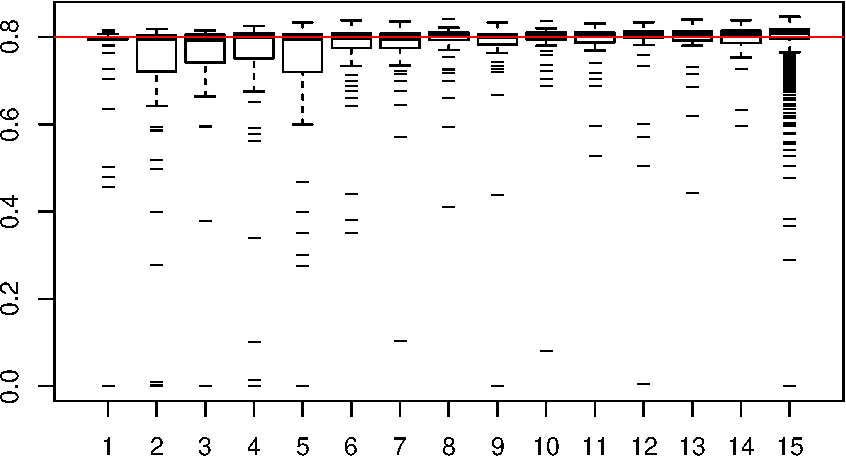
\includegraphics{Figures/unnamed-chunk-6-1.pdf}

\begin{Shaded}
\begin{Highlighting}[]
\KeywordTok{accuracy}\NormalTok{(m4)}
\end{Highlighting}
\end{Shaded}

\begin{verbatim}
## $conf.table
##          actual
## predicted   0   1
##         0 120  61
##         1  11  13
## 
## $precision
## [1] 0.5416667
## 
## $recall
## [1] 0.1756757
\end{verbatim}

This identification result holds under the assumption that the skill
distribution is logistic. Next, we relax this distributional assumption.
First, we check different distributions {[}e.g., probit, cauchit,
cloglog{]}. Second, we estimate the parameter with non-parametric binary
regression models, such as Klein and Spady.

\begin{Shaded}
\begin{Highlighting}[]
\CommentTok{# Not sure about this implementation!}
\KeywordTok{require}\NormalTok{(np)}
\NormalTok{m.np <-}\StringTok{ }\KeywordTok{npindexbw}\NormalTok{(}\KeywordTok{as.numeric}\NormalTok{(submit) }\OperatorTok{~}\StringTok{ }\NormalTok{rating }\OperatorTok{+}\StringTok{ }\NormalTok{lhours.imp }\OperatorTok{+}\StringTok{ }
\StringTok{    }\NormalTok{treatment, }\DataTypeTok{data =}\NormalTok{ dat, }\DataTypeTok{method =} \StringTok{"kleinspady"}\NormalTok{)}
\end{Highlighting}
\end{Shaded}

\begin{verbatim}
## Error in npindexbw(as.numeric(submit) ~ rating + lhours.imp + treatment, : could not find function "is"
\end{verbatim}

\begin{Shaded}
\begin{Highlighting}[]
\KeywordTok{summary}\NormalTok{(m.np)}
\end{Highlighting}
\end{Shaded}

\begin{verbatim}
## Error in summary(m.np): object 'm.np' not found
\end{verbatim}

\begin{Shaded}
\begin{Highlighting}[]
\CommentTok{# plot(m.np)}
\end{Highlighting}
\end{Shaded}

We find that ``ratings'' and ``hours'' are strong predictors of entry.
Yet, precision of the predictions seems pretty low using GLM. Fit does
not seem change much if we use more flexible non-parametric models, such
as GAMs.

\begin{Shaded}
\begin{Highlighting}[]
\CommentTok{# Baseline Binomial model [odds(y) = exp(alpha_i + beta *}
\CommentTok{# rating)]}
\NormalTok{baseline <-}\StringTok{ }\KeywordTok{glm}\NormalTok{(submit }\OperatorTok{~}\StringTok{ }\NormalTok{treatment, }\KeywordTok{binomial}\NormalTok{(logit), }\DataTypeTok{data =}\NormalTok{ dat)}
\KeywordTok{summary}\NormalTok{(baseline)}
\end{Highlighting}
\end{Shaded}

\begin{verbatim}
## 
## Call:
## glm(formula = submit ~ treatment, family = binomial(logit), data = dat)
## 
## Deviance Residuals: 
##     Min       1Q   Median       3Q      Max  
## -0.8950  -0.7934  -0.7806   1.4891   1.6353  
## 
## Coefficients:
##                     Estimate Std. Error z value Pr(>|z|)    
## (Intercept)         -1.03236    0.22839  -4.520 6.18e-06 ***
## treatmenttournament  0.32418    0.31207   1.039    0.299    
## treatmentreserve     0.03774    0.32077   0.118    0.906    
## ---
## Signif. codes:  0 '***' 0.001 '**' 0.01 '*' 0.05 '.' 0.1 ' ' 1
## 
## (Dispersion parameter for binomial family taken to be 1)
## 
##     Null deviance: 358.81  on 298  degrees of freedom
## Residual deviance: 357.49  on 296  degrees of freedom
## AIC: 363.49
## 
## Number of Fisher Scoring iterations: 4
\end{verbatim}

\begin{Shaded}
\begin{Highlighting}[]
\CommentTok{# Overfitted model}
\NormalTok{overfit <-}\StringTok{ }\KeywordTok{glm}\NormalTok{(submit }\OperatorTok{~}\StringTok{ }\NormalTok{., }\KeywordTok{binomial}\NormalTok{(logit), }\DataTypeTok{data =}\NormalTok{ dat)}
\KeywordTok{summary}\NormalTok{(overfit)}
\end{Highlighting}
\end{Shaded}

\begin{verbatim}
## 
## Call:
## glm(formula = submit ~ ., family = binomial(logit), data = dat)
## 
## Deviance Residuals: 
##     Min       1Q   Median       3Q      Max  
## -1.7359  -0.9241  -0.6957   1.2417   1.8804  
## 
## Coefficients:
##                      Estimate Std. Error z value Pr(>|z|)  
## (Intercept)         -27.41859   94.12777  -0.291   0.7708  
## treatmenttournament   0.26901    0.37744   0.713   0.4760  
## treatmentreserve      0.19883    0.37800   0.526   0.5989  
## rating                0.08958    0.05075   1.765   0.0775 .
## nwins                -0.16805    0.17948  -0.936   0.3491  
## ntop10                0.05833    0.07067   0.825   0.4091  
## year                  0.01233    0.04690   0.263   0.7927  
## month                 0.04605    0.04535   1.015   0.3099  
## lhours.imp            0.50449    0.24760   2.038   0.0416 *
## risk.imp             -0.01388    0.07071  -0.196   0.8444  
## timezone.imp         -0.01496    0.03045  -0.491   0.6232  
## ---
## Signif. codes:  0 '***' 0.001 '**' 0.01 '*' 0.05 '.' 0.1 ' ' 1
## 
## (Dispersion parameter for binomial family taken to be 1)
## 
##     Null deviance: 268.13  on 204  degrees of freedom
## Residual deviance: 251.26  on 194  degrees of freedom
##   (94 observations deleted due to missingness)
## AIC: 273.26
## 
## Number of Fisher Scoring iterations: 4
\end{verbatim}

\begin{Shaded}
\begin{Highlighting}[]
\CommentTok{# Model selection}
\NormalTok{selmodel <-}\StringTok{ }\KeywordTok{step}\NormalTok{(overfit)}
\end{Highlighting}
\end{Shaded}

\begin{verbatim}
## Start:  AIC=273.26
## submit ~ treatment + rating + nwins + ntop10 + year + month + 
##     lhours.imp + risk.imp + timezone.imp
## 
##                Df Deviance    AIC
## - treatment     2   251.81 269.81
## - risk.imp      1   251.30 271.30
## - year          1   251.33 271.33
## - timezone.imp  1   251.50 271.50
## - ntop10        1   251.95 271.95
## - nwins         1   252.15 272.15
## - month         1   252.29 272.29
## <none>              251.26 273.26
## - rating        1   254.44 274.44
## - lhours.imp    1   255.59 275.59
## 
## Step:  AIC=269.81
## submit ~ rating + nwins + ntop10 + year + month + lhours.imp + 
##     risk.imp + timezone.imp
## 
##                Df Deviance    AIC
## - risk.imp      1   251.84 267.83
## - year          1   251.89 267.89
## - timezone.imp  1   252.06 268.06
## - ntop10        1   252.47 268.47
## - nwins         1   252.71 268.71
## - month         1   252.97 268.97
## <none>              251.81 269.81
## - rating        1   255.08 271.08
## - lhours.imp    1   256.10 272.10
## 
## Step:  AIC=267.84
## submit ~ rating + nwins + ntop10 + year + month + lhours.imp + 
##     timezone.imp
## 
##                Df Deviance    AIC
## - year          1   251.91 265.91
## - timezone.imp  1   252.11 266.11
## - ntop10        1   252.50 266.50
## - nwins         1   252.75 266.75
## - month         1   252.98 266.98
## <none>              251.84 267.83
## - rating        1   255.29 269.29
## - lhours.imp    1   256.16 270.16
## 
## Step:  AIC=265.91
## submit ~ rating + nwins + ntop10 + month + lhours.imp + timezone.imp
## 
##                Df Deviance    AIC
## - timezone.imp  1   252.16 264.16
## - ntop10        1   252.53 264.53
## - nwins         1   252.79 264.79
## - month         1   252.99 264.99
## <none>              251.91 265.91
## - rating        1   255.36 267.36
## - lhours.imp    1   256.55 268.55
## 
## Step:  AIC=264.16
## submit ~ rating + nwins + ntop10 + month + lhours.imp
## 
##              Df Deviance    AIC
## - ntop10      1   252.75 262.75
## - nwins       1   253.02 263.02
## - month       1   253.25 263.25
## <none>            252.16 264.16
## - rating      1   255.51 265.51
## - lhours.imp  1   256.64 266.64
## 
## Step:  AIC=262.75
## submit ~ rating + nwins + month + lhours.imp
## 
##              Df Deviance    AIC
## - nwins       1   253.04 261.04
## - month       1   253.75 261.75
## <none>            252.75 262.75
## - lhours.imp  1   257.10 265.10
## - rating      1   260.16 268.16
## 
## Step:  AIC=261.04
## submit ~ rating + month + lhours.imp
## 
##              Df Deviance    AIC
## - month       1   253.96 259.96
## <none>            253.04 261.04
## - lhours.imp  1   257.76 263.76
## - rating      1   260.92 266.92
## 
## Step:  AIC=259.96
## submit ~ rating + lhours.imp
## 
##              Df Deviance    AIC
## <none>            253.96 259.96
## - lhours.imp  1   259.15 263.15
## - rating      1   263.41 267.41
\end{verbatim}

\begin{Shaded}
\begin{Highlighting}[]
\KeywordTok{summary}\NormalTok{(selmodel)}
\end{Highlighting}
\end{Shaded}

\begin{verbatim}
## 
## Call:
## glm(formula = submit ~ rating + lhours.imp, family = binomial(logit), 
##     data = dat)
## 
## Deviance Residuals: 
##     Min       1Q   Median       3Q      Max  
## -1.6527  -0.9318  -0.7466   1.2577   1.7707  
## 
## Coefficients:
##             Estimate Std. Error z value Pr(>|z|)   
## (Intercept) -2.30967    0.77498  -2.980  0.00288 **
## rating       0.10813    0.03632   2.978  0.00290 **
## lhours.imp   0.51926    0.23353   2.224  0.02618 * 
## ---
## Signif. codes:  0 '***' 0.001 '**' 0.01 '*' 0.05 '.' 0.1 ' ' 1
## 
## (Dispersion parameter for binomial family taken to be 1)
## 
##     Null deviance: 268.13  on 204  degrees of freedom
## Residual deviance: 253.96  on 202  degrees of freedom
##   (94 observations deleted due to missingness)
## AIC: 259.96
## 
## Number of Fisher Scoring iterations: 4
\end{verbatim}

\begin{Shaded}
\begin{Highlighting}[]
\CommentTok{# Try different symmetric and non-symmetric distributions}
\NormalTok{probit <-}\StringTok{ }\KeywordTok{update}\NormalTok{(selmodel, }\DataTypeTok{family =} \KeywordTok{binomial}\NormalTok{(probit))}
\NormalTok{cauchit <-}\StringTok{ }\KeywordTok{update}\NormalTok{(selmodel, }\DataTypeTok{family =} \KeywordTok{binomial}\NormalTok{(cauchit))}
\NormalTok{cloglog <-}\StringTok{ }\KeywordTok{update}\NormalTok{(selmodel, }\DataTypeTok{family =} \KeywordTok{binomial}\NormalTok{(cloglog))}

\CommentTok{# What model to choose?}
\NormalTok{fit <-}\StringTok{ }\KeywordTok{list}\NormalTok{(}\DataTypeTok{logit =}\NormalTok{ selmodel, }\DataTypeTok{probit =}\NormalTok{ probit, }\DataTypeTok{cauchit =}\NormalTok{ cauchit, }
    \DataTypeTok{cloglog =}\NormalTok{ cloglog)}
\KeywordTok{cbind}\NormalTok{(}\DataTypeTok{deviance =} \KeywordTok{sapply}\NormalTok{(fit, deviance), }\DataTypeTok{n =} \KeywordTok{sapply}\NormalTok{(fit, }\ControlFlowTok{function}\NormalTok{(x) }\KeywordTok{length}\NormalTok{(x}\OperatorTok{$}\NormalTok{y)))}
\end{Highlighting}
\end{Shaded}

\begin{verbatim}
##         deviance   n
## logit   253.9631 205
## probit  253.7955 205
## cauchit 254.8235 205
## cloglog 254.4793 205
\end{verbatim}

\begin{Shaded}
\begin{Highlighting}[]
\CommentTok{# Probit seems to be better}

\CommentTok{# Precision?}
\NormalTok{accuracy <-}\StringTok{ }\ControlFlowTok{function}\NormalTok{(fit) \{}
\NormalTok{    yhat <-}\StringTok{ }\KeywordTok{predict}\NormalTok{(fit, }\DataTypeTok{type =} \StringTok{"response"}\NormalTok{)}
\NormalTok{    tab <-}\StringTok{ }\KeywordTok{table}\NormalTok{(}\DataTypeTok{predicted =} \KeywordTok{ifelse}\NormalTok{(yhat }\OperatorTok{>}\StringTok{ }\FloatTok{0.5}\NormalTok{, }\DecValTok{1}\NormalTok{, }\DecValTok{0}\NormalTok{), }\DataTypeTok{actual =}\NormalTok{ fit}\OperatorTok{$}\NormalTok{y)}
\NormalTok{    tp <-}\StringTok{ }\NormalTok{tab[}\DecValTok{2}\NormalTok{, }\DecValTok{2}\NormalTok{]}
\NormalTok{    fp <-}\StringTok{ }\NormalTok{tab[}\DecValTok{2}\NormalTok{, }\DecValTok{1}\NormalTok{]}
\NormalTok{    fn <-}\StringTok{ }\NormalTok{tab[}\DecValTok{1}\NormalTok{, }\DecValTok{2}\NormalTok{]}
\NormalTok{    precision <-}\StringTok{ }\NormalTok{tp}\OperatorTok{/}\NormalTok{(tp }\OperatorTok{+}\StringTok{ }\NormalTok{fp)}
\NormalTok{    recall <-}\StringTok{ }\NormalTok{tp}\OperatorTok{/}\NormalTok{(tp }\OperatorTok{+}\StringTok{ }\NormalTok{fn)}
    \CommentTok{# cat(sprintf('Precision: %0.2f\textbackslash{}nRecall: %0.2f\textbackslash{}n',}
    \CommentTok{# precision, recall))}
    \KeywordTok{list}\NormalTok{(}\DataTypeTok{conf.table =}\NormalTok{ tab, }\DataTypeTok{precision =}\NormalTok{ precision, }\DataTypeTok{recall =}\NormalTok{ recall)}
\NormalTok{\}}
\KeywordTok{accuracy}\NormalTok{(probit)}
\end{Highlighting}
\end{Shaded}

\begin{verbatim}
## $conf.table
##          actual
## predicted   0   1
##         0 122  60
##         1   9  14
## 
## $precision
## [1] 0.6086957
## 
## $recall
## [1] 0.1891892
\end{verbatim}

\begin{Shaded}
\begin{Highlighting}[]
\CommentTok{# Try with treatment interactions}
\NormalTok{probit.interact <-}\StringTok{ }\KeywordTok{update}\NormalTok{(probit, }\StringTok{"~ .*treatment"}\NormalTok{)}
\KeywordTok{summary}\NormalTok{(probit.interact)}
\end{Highlighting}
\end{Shaded}

\begin{verbatim}
## 
## Call:
## glm(formula = submit ~ rating + lhours.imp + treatment + rating:treatment + 
##     lhours.imp:treatment, family = binomial(probit), data = dat)
## 
## Deviance Residuals: 
##     Min       1Q   Median       3Q      Max  
## -2.1770  -0.9456  -0.6852   1.2793   1.9389  
## 
## Coefficients:
##                                Estimate Std. Error z value Pr(>|z|)  
## (Intercept)                    -2.15032    0.88844  -2.420   0.0155 *
## rating                          0.07513    0.03881   1.936   0.0529 .
## lhours.imp                      0.50789    0.26691   1.903   0.0571 .
## treatmenttournament             0.12043    1.19785   0.101   0.9199  
## treatmentreserve                2.25059    1.22286   1.840   0.0657 .
## rating:treatmenttournament      0.02969    0.05684   0.522   0.6014  
## rating:treatmentreserve        -0.05994    0.05418  -1.106   0.2687  
## lhours.imp:treatmenttournament  0.01505    0.36034   0.042   0.9667  
## lhours.imp:treatmentreserve    -0.64835    0.37229  -1.742   0.0816 .
## ---
## Signif. codes:  0 '***' 0.001 '**' 0.01 '*' 0.05 '.' 0.1 ' ' 1
## 
## (Dispersion parameter for binomial family taken to be 1)
## 
##     Null deviance: 268.13  on 204  degrees of freedom
## Residual deviance: 246.46  on 196  degrees of freedom
##   (94 observations deleted due to missingness)
## AIC: 264.46
## 
## Number of Fisher Scoring iterations: 5
\end{verbatim}

\begin{Shaded}
\begin{Highlighting}[]
\KeywordTok{accuracy}\NormalTok{(probit.interact)}
\end{Highlighting}
\end{Shaded}

\begin{verbatim}
## $conf.table
##          actual
## predicted   0   1
##         0 122  56
##         1   9  18
## 
## $precision
## [1] 0.6666667
## 
## $recall
## [1] 0.2432432
\end{verbatim}

\begin{Shaded}
\begin{Highlighting}[]
\CommentTok{# Model selection again:}
\KeywordTok{step}\NormalTok{(probit.interact)}
\end{Highlighting}
\end{Shaded}

\begin{verbatim}
## Start:  AIC=264.46
## submit ~ rating + lhours.imp + treatment + rating:treatment + 
##     lhours.imp:treatment
## 
##                        Df Deviance    AIC
## - rating:treatment      2   249.34 263.34
## <none>                      246.46 264.46
## - lhours.imp:treatment  2   250.81 264.81
## 
## Step:  AIC=263.34
## submit ~ rating + lhours.imp + treatment + lhours.imp:treatment
## 
##                        Df Deviance    AIC
## - lhours.imp:treatment  2   253.09 263.09
## <none>                      249.34 263.34
## - rating                1   258.16 270.16
## 
## Step:  AIC=263.09
## submit ~ rating + lhours.imp + treatment
## 
##              Df Deviance    AIC
## - treatment   2   253.80 259.80
## <none>            253.09 263.09
## - lhours.imp  1   258.38 266.38
## - rating      1   262.80 270.80
## 
## Step:  AIC=259.8
## submit ~ rating + lhours.imp
## 
##              Df Deviance    AIC
## <none>            253.80 259.80
## - lhours.imp  1   259.13 263.13
## - rating      1   263.44 267.44
\end{verbatim}

\begin{verbatim}
## 
## Call:  glm(formula = submit ~ rating + lhours.imp, family = binomial(probit), 
##     data = dat)
## 
## Coefficients:
## (Intercept)       rating   lhours.imp  
##     -1.4318       0.0666       0.3223  
## 
## Degrees of Freedom: 204 Total (i.e. Null);  202 Residual
##   (94 observations deleted due to missingness)
## Null Deviance:       268.1 
## Residual Deviance: 253.8     AIC: 259.8
\end{verbatim}

\begin{Shaded}
\begin{Highlighting}[]
\CommentTok{# FIGURE}
\NormalTok{plot.fit <-}\StringTok{ }\ControlFlowTok{function}\NormalTok{(x, ...) \{}
\NormalTok{    yhat <-}\StringTok{ }\KeywordTok{predict}\NormalTok{(x)}
    \KeywordTok{plot}\NormalTok{(}\KeywordTok{jitter}\NormalTok{(yhat), }\KeywordTok{jitter}\NormalTok{(}\KeywordTok{as.numeric}\NormalTok{(x}\OperatorTok{$}\NormalTok{y)), }\DataTypeTok{pch =} \DecValTok{16}\NormalTok{, }\DataTypeTok{col =} \KeywordTok{ifelse}\NormalTok{(yhat }\OperatorTok{>}\StringTok{ }
\StringTok{        }\FloatTok{0.5}\NormalTok{, }\StringTok{"red"}\NormalTok{, }\StringTok{"blue"}\NormalTok{), ...)}
    \KeywordTok{curve}\NormalTok{(ilogit, }\DataTypeTok{add =} \OtherTok{TRUE}\NormalTok{)}
    \KeywordTok{abline}\NormalTok{(}\DataTypeTok{h =} \KeywordTok{c}\NormalTok{(}\DecValTok{0}\NormalTok{, }\DecValTok{1}\NormalTok{), }\DataTypeTok{lty =} \DecValTok{2}\NormalTok{, }\DataTypeTok{col =} \KeywordTok{gray}\NormalTok{(}\FloatTok{0.9}\NormalTok{))}
\NormalTok{\}}
\CommentTok{# par(mfrow=c(3,3), mar=c(2,2,1,1)) sapply(1:length(fit),}
\CommentTok{# function(i) \{ plot.fit(fit[[i]], xlim=c(-3, 3))}
\CommentTok{# title(names(fit)[i]) \})}


\CommentTok{# Regression by treatment}
\NormalTok{fit2 <-}\StringTok{ }\KeywordTok{rep}\NormalTok{()}
\NormalTok{fit2}\OperatorTok{$}\NormalTok{race <-}\StringTok{ }\KeywordTok{glm}\NormalTok{(submit }\OperatorTok{~}\StringTok{ }\NormalTok{rating }\OperatorTok{+}\StringTok{ }\NormalTok{lhours.imp, }\DataTypeTok{data =}\NormalTok{ dat, }\KeywordTok{binomial}\NormalTok{(logit), }
    \DataTypeTok{subset =}\NormalTok{ treatment }\OperatorTok{==}\StringTok{ "race"}\NormalTok{)}
\NormalTok{fit2}\OperatorTok{$}\NormalTok{tourn <-}\StringTok{ }\KeywordTok{glm}\NormalTok{(submit }\OperatorTok{~}\StringTok{ }\NormalTok{rating }\OperatorTok{+}\StringTok{ }\NormalTok{lhours.imp, }\DataTypeTok{data =}\NormalTok{ dat, }\KeywordTok{binomial}\NormalTok{(logit), }
    \DataTypeTok{subset =}\NormalTok{ treatment }\OperatorTok{==}\StringTok{ "tournament"}\NormalTok{)}
\NormalTok{fit2}\OperatorTok{$}\NormalTok{rese <-}\StringTok{ }\KeywordTok{glm}\NormalTok{(submit }\OperatorTok{~}\StringTok{ }\NormalTok{rating }\OperatorTok{+}\StringTok{ }\NormalTok{lhours.imp, }\DataTypeTok{data =}\NormalTok{ dat, }\KeywordTok{binomial}\NormalTok{(logit), }
    \DataTypeTok{subset =}\NormalTok{ treatment }\OperatorTok{==}\StringTok{ "reserve"}\NormalTok{)}

\KeywordTok{stargazer}\NormalTok{(fit2, }\DataTypeTok{type =} \StringTok{"text"}\NormalTok{, }\DataTypeTok{column.labels =} \KeywordTok{names}\NormalTok{(fit2))}
\end{Highlighting}
\end{Shaded}

\begin{verbatim}
## 
## ===============================================
##                        Dependent variable:     
##                   -----------------------------
##                              submit            
##                      race      tourn     rese  
##                      (1)        (2)      (3)   
## -----------------------------------------------
## rating              0.120*    0.187**   0.025  
##                    (0.064)    (0.073)  (0.061) 
##                                                
## lhours.imp          0.813*    0.858**   -0.230 
##                    (0.456)    (0.414)  (0.422) 
##                                                
## Constant           -3.449**  -3.334**   0.175  
##                    (1.534)    (1.384)  (1.361) 
##                                                
## -----------------------------------------------
## Observations          68        69        68   
## Log Likelihood     -39.558    -39.229  -44.455 
## Akaike Inf. Crit.   85.116    84.459    94.909 
## ===============================================
## Note:               *p<0.1; **p<0.05; ***p<0.01
\end{verbatim}

\begin{Shaded}
\begin{Highlighting}[]
\CommentTok{# Plot}
\KeywordTok{par}\NormalTok{(}\DataTypeTok{mfrow =} \KeywordTok{c}\NormalTok{(}\DecValTok{1}\NormalTok{, }\DecValTok{3}\NormalTok{), }\DataTypeTok{mar =} \KeywordTok{c}\NormalTok{(}\DecValTok{2}\NormalTok{, }\DecValTok{2}\NormalTok{, }\DecValTok{1}\NormalTok{, }\DecValTok{1}\NormalTok{))}
\KeywordTok{sapply}\NormalTok{(}\DecValTok{1}\OperatorTok{:}\DecValTok{3}\NormalTok{, }\ControlFlowTok{function}\NormalTok{(i) \{}
    \KeywordTok{plot.fit}\NormalTok{(fit2[[i]], }\DataTypeTok{xlim =} \KeywordTok{c}\NormalTok{(}\OperatorTok{-}\DecValTok{3}\NormalTok{, }\DecValTok{3}\NormalTok{))}
    \KeywordTok{title}\NormalTok{(}\KeywordTok{names}\NormalTok{(fit2)[i])}
\NormalTok{\})}
\end{Highlighting}
\end{Shaded}

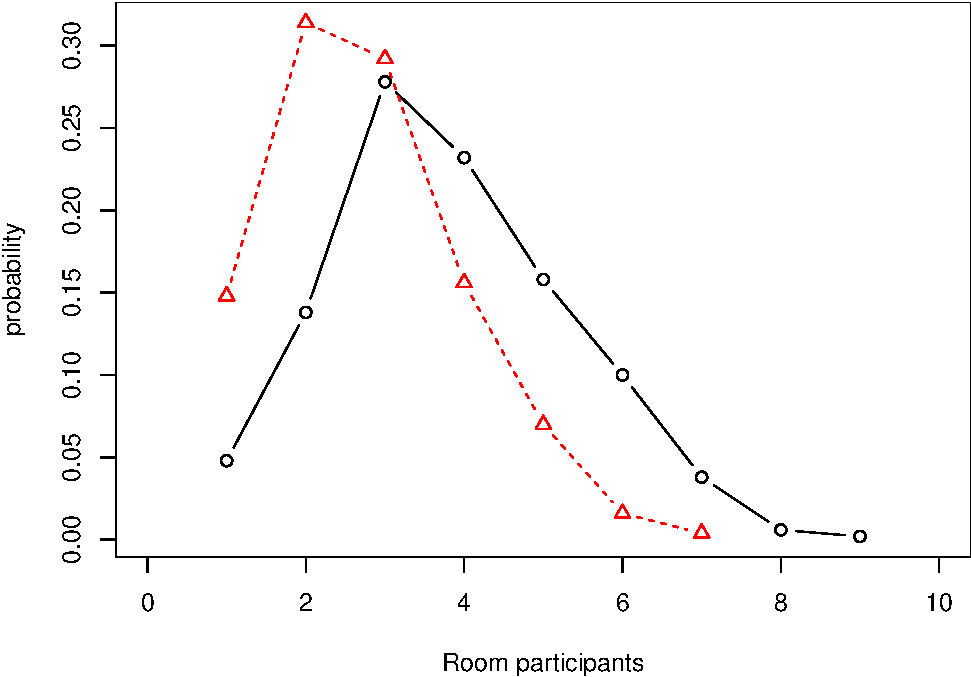
\includegraphics{Figures/unnamed-chunk-8-1.pdf}

\begin{verbatim}
## [[1]]
## NULL
## 
## [[2]]
## NULL
## 
## [[3]]
## NULL
\end{verbatim}

\begin{Shaded}
\begin{Highlighting}[]
\CommentTok{# Bayesian models}
\NormalTok{model <-}\StringTok{ "submit ~ treatment + tothours.imp + mm_rating.100 + educ+gender+timezone"}
\CommentTok{# bayes <- arm::bayesglm(model, family=binomial)}
\CommentTok{# summary(bayes)}

\CommentTok{# Generalized additive models}
\NormalTok{b <-}\StringTok{ }\NormalTok{mgcv}\OperatorTok{::}\KeywordTok{gam}\NormalTok{(submit }\OperatorTok{~}\StringTok{ }\NormalTok{treatment }\OperatorTok{+}\StringTok{ }\KeywordTok{s}\NormalTok{(lhours.imp, rating), }\DataTypeTok{data =}\NormalTok{ dat, }
    \DataTypeTok{family =}\NormalTok{ binomial)}
\KeywordTok{plot}\NormalTok{(b, }\DataTypeTok{pages =} \DecValTok{1}\NormalTok{, }\DataTypeTok{seWithMean =} \OtherTok{TRUE}\NormalTok{)  ## `with intercept' CIs}
\end{Highlighting}
\end{Shaded}

\includegraphics{Figures/unnamed-chunk-8-2.pdf}

\begin{Shaded}
\begin{Highlighting}[]
\NormalTok{mgcv}\OperatorTok{::}\KeywordTok{gam.check}\NormalTok{(b)}
\end{Highlighting}
\end{Shaded}

\includegraphics{Figures/unnamed-chunk-8-3.pdf}

\begin{verbatim}
## 
## Method: UBRE   Optimizer: outer newton
## full convergence after 9 iterations.
## Gradient range [-4.419734e-07,-4.419734e-07]
## (score 0.2842903 & scale 1).
## Hessian positive definite, eigenvalue range [4.419576e-07,4.419576e-07].
## Model rank =  32 / 32 
## 
## Basis dimension (k) checking results. Low p-value (k-index<1) may
## indicate that k is too low, especially if edf is close to k'.
## 
##                          k'    edf k-index p-value
## s(lhours.imp,rating) 29.000  2.000   0.959    0.18
\end{verbatim}

\begin{Shaded}
\begin{Highlighting}[]
\KeywordTok{plot.fit}\NormalTok{(b, }\DataTypeTok{xlim =} \KeywordTok{c}\NormalTok{(}\OperatorTok{-}\DecValTok{3}\NormalTok{, }\DecValTok{3}\NormalTok{))}

\KeywordTok{detach}\NormalTok{(races)}
\end{Highlighting}
\end{Shaded}

\begin{verbatim}
## Error in detach(races): invalid 'name' argument
\end{verbatim}

\includegraphics{Figures/unnamed-chunk-8-4.pdf}

\section{Timing of entry decision using panel
data}\label{timing-of-entry-decision-using-panel-data}

We transform data in a panel with the date of the first submission. The
probability of entry in a given date is modeled with a conditional
logit. We find that the probability of entry in a given date decreases
over time. (if it was at random 1/8 chances of having a submission in a
given date). The estimated drop is about 13 percent from one date to the
next (a reduction of above 100\% from the first to the last date). Using
interactions with treatment dummies, we find that the decrease in the
probability of entry is negative in all treatments but it is about 25
percent in the race (with pvalue\textless{}0.05) it is only 8 (pval) and
6 (pval) percent for tournaments and reserve, respectively.

\begin{Shaded}
\begin{Highlighting}[]
\KeywordTok{rm}\NormalTok{(}\DataTypeTok{list =} \KeywordTok{ls}\NormalTok{())}
\KeywordTok{require}\NormalTok{(magrittr)}
\KeywordTok{require}\NormalTok{(survival)}
\KeywordTok{require}\NormalTok{(races)}
\KeywordTok{data}\NormalTok{(scores)}

\CommentTok{# Create variable}
\NormalTok{dmin <-}\StringTok{ }\ControlFlowTok{function}\NormalTok{(x) x }\OperatorTok{-}\StringTok{ }\KeywordTok{min}\NormalTok{(x)}
\NormalTok{scores}\OperatorTok{$}\NormalTok{date <-}\StringTok{ }\NormalTok{scores}\OperatorTok{$}\NormalTok{timestamp }\OperatorTok\StringTok{ }\NormalTok{as.Date }\OperatorTok\StringTok{ }\NormalTok{as.numeric }\OperatorTok\StringTok{ }
\StringTok{    }\NormalTok{dmin}

\NormalTok{create.panel <-}\StringTok{ }\ControlFlowTok{function}\NormalTok{(data) \{}
\NormalTok{    data}\OperatorTok{$}\NormalTok{submit_first <-}\StringTok{ }\DecValTok{1}
\NormalTok{    g <-}\StringTok{ }\KeywordTok{with}\NormalTok{(data, }\KeywordTok{expand.grid}\NormalTok{(}\DataTypeTok{date =} \KeywordTok{seq}\NormalTok{(}\KeywordTok{min}\NormalTok{(date), }\KeywordTok{max}\NormalTok{(date)), }
        \DataTypeTok{coder_id =} \KeywordTok{unique}\NormalTok{(coder_id), }\DataTypeTok{submit_first =} \DecValTok{0}\NormalTok{))}
\NormalTok{    g2 <-}\StringTok{ }\KeywordTok{rbind}\NormalTok{(g, data[, }\KeywordTok{c}\NormalTok{(}\StringTok{"date"}\NormalTok{, }\StringTok{"coder_id"}\NormalTok{, }\StringTok{"submit_first"}\NormalTok{)])}
    \KeywordTok{aggregate}\NormalTok{(submit_first }\OperatorTok{~}\StringTok{ }\NormalTok{date }\OperatorTok{+}\StringTok{ }\NormalTok{coder_id, g2, }\DataTypeTok{FUN =}\NormalTok{ sum)}
\NormalTok{\}}

\NormalTok{scores.panel <-}\StringTok{ }\KeywordTok{create.panel}\NormalTok{(}\KeywordTok{subset}\NormalTok{(scores, submission }\OperatorTok{==}\StringTok{ }\DecValTok{1}\NormalTok{))}
\NormalTok{z <-}\StringTok{ }\KeywordTok{merge}\NormalTok{(scores.panel, races, }\DataTypeTok{by =} \StringTok{"coder_id"}\NormalTok{)}


\CommentTok{# Unconditional semi-parametric [Odds(first) = exp(alpha +}
\CommentTok{# beta * t )]}
\NormalTok{fit <-}\StringTok{ }\KeywordTok{rep}\NormalTok{()}
\NormalTok{fit}\OperatorTok{$}\NormalTok{clog <-}\StringTok{ }\KeywordTok{clogit}\NormalTok{(submit_first }\OperatorTok{~}\StringTok{ }\NormalTok{date, }\DataTypeTok{data =}\NormalTok{ z)}
\KeywordTok{summary}\NormalTok{(fit}\OperatorTok{$}\NormalTok{clog)}
\end{Highlighting}
\end{Shaded}

\begin{verbatim}
## Call:
## coxph(formula = Surv(rep(1, 774L), submit_first) ~ date, data = z, 
##     method = "exact")
## 
##   n= 774, number of events= 86 
## 
##         coef exp(coef) se(coef)      z Pr(>|z|)   
## date -0.1510    0.8598   0.0461 -3.275  0.00106 **
## ---
## Signif. codes:  0 '***' 0.001 '**' 0.01 '*' 0.05 '.' 0.1 ' ' 1
## 
##      exp(coef) exp(-coef) lower .95 upper .95
## date    0.8598      1.163    0.7855    0.9412
## 
## Rsquare= 0.014   (max possible= 0.498 )
## Likelihood ratio test= 11.17  on 1 df,   p=0.0008303
## Wald test            = 10.73  on 1 df,   p=0.001055
## Score (logrank) test = 11.02  on 1 df,   p=0.0008998
\end{verbatim}

\begin{Shaded}
\begin{Highlighting}[]
\CommentTok{# Unconditional parametric [Odds(first) = exp(alpha + beta *}
\CommentTok{# t )]}
\NormalTok{fit}\OperatorTok{$}\NormalTok{logi <-}\StringTok{ }\KeywordTok{glm}\NormalTok{(submit_first }\OperatorTok{~}\StringTok{ }\NormalTok{date, }\DataTypeTok{data =}\NormalTok{ z, }\KeywordTok{binomial}\NormalTok{(logit))}
\KeywordTok{summary}\NormalTok{(fit}\OperatorTok{$}\NormalTok{logi)}
\end{Highlighting}
\end{Shaded}

\begin{verbatim}
## 
## Call:
## glm(formula = submit_first ~ date, family = binomial(logit), 
##     data = z)
## 
## Deviance Residuals: 
##     Min       1Q   Median       3Q      Max  
## -0.6252  -0.5441  -0.4394  -0.3801   2.3687  
## 
## Coefficients:
##             Estimate Std. Error z value Pr(>|z|)    
## (Intercept) -1.53318    0.18853  -8.132 4.21e-16 ***
## date        -0.15121    0.04614  -3.277  0.00105 ** 
## ---
## Signif. codes:  0 '***' 0.001 '**' 0.01 '*' 0.05 '.' 0.1 ' ' 1
## 
## (Dispersion parameter for binomial family taken to be 1)
## 
##     Null deviance: 539.99  on 773  degrees of freedom
## Residual deviance: 528.81  on 772  degrees of freedom
## AIC: 532.81
## 
## Number of Fisher Scoring iterations: 5
\end{verbatim}

\begin{Shaded}
\begin{Highlighting}[]
\CommentTok{# Unconditional with interaction}
\NormalTok{fit}\OperatorTok{$}\NormalTok{logi2 <-}\StringTok{ }\KeywordTok{glm}\NormalTok{(submit_first }\OperatorTok{~}\StringTok{ }\NormalTok{date }\OperatorTok{+}\StringTok{ }\NormalTok{date}\OperatorTok{:}\NormalTok{treatment, }\DataTypeTok{data =}\NormalTok{ z, }
    \KeywordTok{binomial}\NormalTok{(logit))}
\KeywordTok{summary}\NormalTok{(fit}\OperatorTok{$}\NormalTok{logi2)}
\end{Highlighting}
\end{Shaded}

\begin{verbatim}
## 
## Call:
## glm(formula = submit_first ~ date + date:treatment, family = binomial(logit), 
##     data = z)
## 
## Deviance Residuals: 
##     Min       1Q   Median       3Q      Max  
## -0.6267  -0.5273  -0.4601  -0.3801   2.5737  
## 
## Coefficients:
##                          Estimate Std. Error z value Pr(>|z|)    
## (Intercept)              -1.52808    0.18858  -8.103 5.36e-16 ***
## date                     -0.21835    0.07201  -3.032  0.00243 ** 
## date:treatmenttournament  0.08546    0.07472   1.144  0.25273    
## date:treatmentreserve     0.09344    0.07689   1.215  0.22423    
## ---
## Signif. codes:  0 '***' 0.001 '**' 0.01 '*' 0.05 '.' 0.1 ' ' 1
## 
## (Dispersion parameter for binomial family taken to be 1)
## 
##     Null deviance: 539.99  on 773  degrees of freedom
## Residual deviance: 526.96  on 770  degrees of freedom
## AIC: 534.96
## 
## Number of Fisher Scoring iterations: 5
\end{verbatim}

\begin{Shaded}
\begin{Highlighting}[]
\CommentTok{# Note the difference when the intercept is not there}

\CommentTok{# Conditional [Odds(first) = exp(alpha_i + beta * t )]}
\NormalTok{fit}\OperatorTok{$}\NormalTok{coclog <-}\StringTok{ }\KeywordTok{clogit}\NormalTok{(submit_first }\OperatorTok{~}\StringTok{ }\NormalTok{date }\OperatorTok{+}\StringTok{ }\KeywordTok{strata}\NormalTok{(coder_id), }
    \DataTypeTok{data =}\NormalTok{ z)}
\KeywordTok{summary}\NormalTok{(fit}\OperatorTok{$}\NormalTok{coclog)}
\end{Highlighting}
\end{Shaded}

\begin{verbatim}
## Call:
## coxph(formula = Surv(rep(1, 774L), submit_first) ~ date + strata(coder_id), 
##     data = z, method = "exact")
## 
##   n= 774, number of events= 86 
## 
##         coef exp(coef) se(coef)      z Pr(>|z|)   
## date -0.1340    0.8746   0.0433 -3.095  0.00197 **
## ---
## Signif. codes:  0 '***' 0.001 '**' 0.01 '*' 0.05 '.' 0.1 ' ' 1
## 
##      exp(coef) exp(-coef) lower .95 upper .95
## date    0.8746      1.143    0.8034    0.9521
## 
## Rsquare= 0.013   (max possible= 0.386 )
## Likelihood ratio test= 9.93  on 1 df,   p=0.001627
## Wald test            = 9.58  on 1 df,   p=0.00197
## Score (logrank) test = 9.81  on 1 df,   p=0.001735
\end{verbatim}

\begin{Shaded}
\begin{Highlighting}[]
\CommentTok{# Interactions with treatment dummies [Odds(first) =}
\CommentTok{# exp(alpha_i + beta_i * t )]}
\NormalTok{fit}\OperatorTok{$}\NormalTok{coclog2 <-}\StringTok{ }\KeywordTok{clogit}\NormalTok{(submit_first }\OperatorTok{~}\StringTok{ }\NormalTok{date}\OperatorTok{:}\NormalTok{treatment }\OperatorTok{+}\StringTok{ }\KeywordTok{strata}\NormalTok{(coder_id), }
    \DataTypeTok{data =}\NormalTok{ z)}
\KeywordTok{summary}\NormalTok{(fit}\OperatorTok{$}\NormalTok{coclog2)}
\end{Highlighting}
\end{Shaded}

\begin{verbatim}
## Call:
## coxph(formula = Surv(rep(1, 774L), submit_first) ~ date:treatment + 
##     strata(coder_id), data = z, method = "exact")
## 
##   n= 774, number of events= 86 
## 
##                              coef exp(coef) se(coef)      z Pr(>|z|)   
## date:treatmentrace       -0.27991   0.75585  0.08801 -3.180  0.00147 **
## date:treatmenttournament -0.08726   0.91644  0.06847 -1.274  0.20253   
## date:treatmentreserve    -0.06708   0.93512  0.07522 -0.892  0.37256   
## ---
## Signif. codes:  0 '***' 0.001 '**' 0.01 '*' 0.05 '.' 0.1 ' ' 1
## 
##                          exp(coef) exp(-coef) lower .95 upper .95
## date:treatmentrace          0.7559      1.323    0.6361    0.8982
## date:treatmenttournament    0.9164      1.091    0.8013    1.0481
## date:treatmentreserve       0.9351      1.069    0.8069    1.0837
## 
## Rsquare= 0.018   (max possible= 0.386 )
## Likelihood ratio test= 14.16  on 3 df,   p=0.002689
## Wald test            = 12.53  on 3 df,   p=0.005761
## Score (logrank) test = 13.61  on 3 df,   p=0.003487
\end{verbatim}

\begin{Shaded}
\begin{Highlighting}[]
\CommentTok{# Note: the above model is the same as clogit(submit_first ~}
\CommentTok{# date + date:treatment + strata(coder_id), data=z)}

\CommentTok{# Coefficients}
\KeywordTok{sapply}\NormalTok{(fit, coef)}
\end{Highlighting}
\end{Shaded}

\begin{verbatim}
## $clog
##       date 
## -0.1510078 
## 
## $logi
## (Intercept)        date 
##  -1.5331826  -0.1512076 
## 
## $logi2
##              (Intercept)                     date date:treatmenttournament 
##              -1.52808481              -0.21835013               0.08545552 
##    date:treatmentreserve 
##               0.09344282 
## 
## $coclog
##       date 
## -0.1339918 
## 
## $coclog2
##       date:treatmentrace date:treatmenttournament    date:treatmentreserve 
##              -0.27990753              -0.08725850              -0.06707555
\end{verbatim}

\begin{Shaded}
\begin{Highlighting}[]
\CommentTok{# Days as factors}


\CommentTok{# # Compute first submission time time.max <- '2015-03-16}
\CommentTok{# 11:59:59 EDT' time.min <- '2015-03-08 12:00:00 EDT'}
\CommentTok{# time.censored <- 192 fsutime <-}
\CommentTok{# as.numeric(difftime(races.sub$timestamp, time.min ,}
\CommentTok{# unit='hours')) dat <- with(races.sub, aggregate(fsutime ~}
\CommentTok{# handle, FUN=min)) dat$fsu <- 1 dat2 <- merge(dat, races,}
\CommentTok{# by='handle', all=TRUE) dat2$fsu[is.na(dat2$fsu)] <- 0}
\CommentTok{# dat2$fsutime[is.na(dat2$fsutime)] <- time.censored surv <-}
\CommentTok{# rep() surv$m1 <- survreg(Surv(fsutime, fsu) ~ 1, dat2,}
\CommentTok{# dist='weibull', scale=1) surv$m2 <- survreg(Surv(fsutime,}
\CommentTok{# fsu) ~ treatment + mmevents, dat2 , dist='weibull',}
\CommentTok{# scale=1) surv$m3 <- survreg(Surv(fsutime, fsu) ~ treatment}
\CommentTok{# + mmevents, dat2, dist='exponential') surv$tobin <-}
\CommentTok{# survreg(Surv(fsutime, fsu, type='left') ~ treatment +}
\CommentTok{# mmevents, data=dat2, dist='gaussian') stargazer(surv,}
\CommentTok{# type='text') # A model with different baseline survival}
\CommentTok{# shapes for two groups, i.e., # two different scale}
\CommentTok{# parameters survreg(Surv(time, status) ~ ph.ecog + age +}
\CommentTok{# strata(sex), lung) # There are multiple ways to}
\CommentTok{# parameterize a Weibull distribution. The survreg # function}
\CommentTok{# embeds it in a general location-scale family, which is a #}
\CommentTok{# different parameterization than the rweibull function, and}
\CommentTok{# often leads # to confusion.  # survreg's scale =}
\CommentTok{# 1/(rweibull shape) # survreg's intercept = log(rweibull}
\CommentTok{# scale) # For the log-likelihood all parameterizations lead}
\CommentTok{# to the same value.  y <- rweibull(1000, shape=2, scale=5)}
\CommentTok{# survreg(Surv(y)~1, dist='weibull') # Economists fit a model}
\CommentTok{# called `tobit regression', which is a standard # linear}
\CommentTok{# regression with Gaussian errors, and left censored data.}
\CommentTok{# tobinfit <- survreg(Surv(durable, durable>0, type='left') ~}
\CommentTok{# age + quant, data=tobin, dist='gaussian')}
\end{Highlighting}
\end{Shaded}

\section{Analysis of scores}\label{analysis-of-scores}

As a measure of the ability to make correct predictions of domain expert
annotations we used the ``F-score'' defined as the harmonic mean of
precision and recall:
\(F = 2 * (precision * recall) / (precision + recall)\)). This score was
computed on 300 abstracts (100 of which were not disculosed to avoid
overfitting) with about xxxx entities to correctly identify from a
dictionary with xxxx labels.

\begin{Shaded}
\begin{Highlighting}[]
\NormalTok{baseline <-}\StringTok{ }\FloatTok{0.792867}
\NormalTok{target <-}\StringTok{ }\FloatTok{0.817866}
\NormalTok{winner <-}\StringTok{ }\FloatTok{0.843962}
\end{Highlighting}
\end{Shaded}

The baseline F-score achieved by NIH researchers was 0.792867. We set up
a hard-to-reach F-score target for the race competition which was
0.817866 (about a 3 percent increase of the baseline). The winner
achieved a score of 0.843962. This represents a 5.1095 percentage points
increase compared to the baseline which can be regarded as a very
remarkable improvement (more than 6 percent).

Figure below shows the provisional scores over the submission time. The
left panel shows the raw scores that are very volitile because some
preliminary submissions failed to compile or encountered other issues
that either terminated the program resulting in a zero or lead to very
low scores. This high volatility, however, does not reflect genuine
variation in the quality of submissions. The right panel shows the
scores capped from {[}below to reduce volatility due to experimentation
with imperfect solutions{]}.

\begin{Shaded}
\begin{Highlighting}[]
\CommentTok{# Load libraries}
\KeywordTok{require}\NormalTok{(races)}
\KeywordTok{require}\NormalTok{(stargazer)}
\CommentTok{# require(mgcv) require(arm)}

\CommentTok{# Load Data}
\KeywordTok{data}\NormalTok{(races)}
\KeywordTok{data}\NormalTok{(scores)}

\CommentTok{# Merge}
\NormalTok{dat <-}\StringTok{ }\KeywordTok{merge}\NormalTok{(scores, races[, }\KeywordTok{c}\NormalTok{(}\StringTok{"coder_id"}\NormalTok{, }\StringTok{"treatment"}\NormalTok{, }\StringTok{"room"}\NormalTok{)], }
    \DataTypeTok{by =} \StringTok{"coder_id"}\NormalTok{)}
\NormalTok{dat <-}\StringTok{ }\NormalTok{dat[}\KeywordTok{order}\NormalTok{(dat}\OperatorTok{$}\NormalTok{timestamp), ]}

\KeywordTok{attach}\NormalTok{(dat)}
\NormalTok{provisional <-}\StringTok{ }\NormalTok{provisional}\OperatorTok{/}\FloatTok{1e+06}
\NormalTok{final <-}\StringTok{ }\NormalTok{final}\OperatorTok{/}\FloatTok{1e+06}
\NormalTok{hours <-}\StringTok{ }\KeywordTok{as.numeric}\NormalTok{(}\KeywordTok{difftime}\NormalTok{(timestamp, }\KeywordTok{min}\NormalTok{(timestamp), }\DataTypeTok{unit =} \StringTok{"hours"}\NormalTok{))}

\CommentTok{# New variable}
\NormalTok{last_submission <-}\StringTok{ }\KeywordTok{ave}\NormalTok{(submission, coder_id, }\DataTypeTok{FUN =}\NormalTok{ max)}
\NormalTok{provisional.cap <-}\StringTok{ }\KeywordTok{ifelse}\NormalTok{(provisional }\OperatorTok{<}\StringTok{ }\NormalTok{baseline, baseline, provisional)}
\NormalTok{final.cap <-}\StringTok{ }\KeywordTok{ifelse}\NormalTok{(final }\OperatorTok{<}\StringTok{ }\NormalTok{baseline, baseline, final)}


\CommentTok{# General plot}
\KeywordTok{par}\NormalTok{(}\DataTypeTok{mfrow =} \KeywordTok{c}\NormalTok{(}\DecValTok{1}\NormalTok{, }\DecValTok{2}\NormalTok{))}
\KeywordTok{plot}\NormalTok{(}\KeywordTok{aggregate}\NormalTok{(final }\OperatorTok{~}\StringTok{ }\NormalTok{hours, }\DataTypeTok{FUN =}\NormalTok{ mean), }\DataTypeTok{type =} \StringTok{"l"}\NormalTok{, }\DataTypeTok{lwd =} \DecValTok{2}\NormalTok{, }
    \DataTypeTok{col =} \KeywordTok{gray}\NormalTok{(}\FloatTok{0.85}\NormalTok{))}
\KeywordTok{plot}\NormalTok{(}\KeywordTok{aggregate}\NormalTok{(final.cap }\OperatorTok{~}\StringTok{ }\NormalTok{hours, }\DataTypeTok{FUN =}\NormalTok{ mean), }\DataTypeTok{type =} \StringTok{"l"}\NormalTok{, }\DataTypeTok{lwd =} \DecValTok{2}\NormalTok{, }
    \DataTypeTok{col =} \KeywordTok{gray}\NormalTok{(}\FloatTok{0.85}\NormalTok{))}
\KeywordTok{abline}\NormalTok{(}\DataTypeTok{h =}\NormalTok{ target, }\DataTypeTok{lty =} \DecValTok{2}\NormalTok{, }\DataTypeTok{col =} \DecValTok{2}\NormalTok{)}
\end{Highlighting}
\end{Shaded}

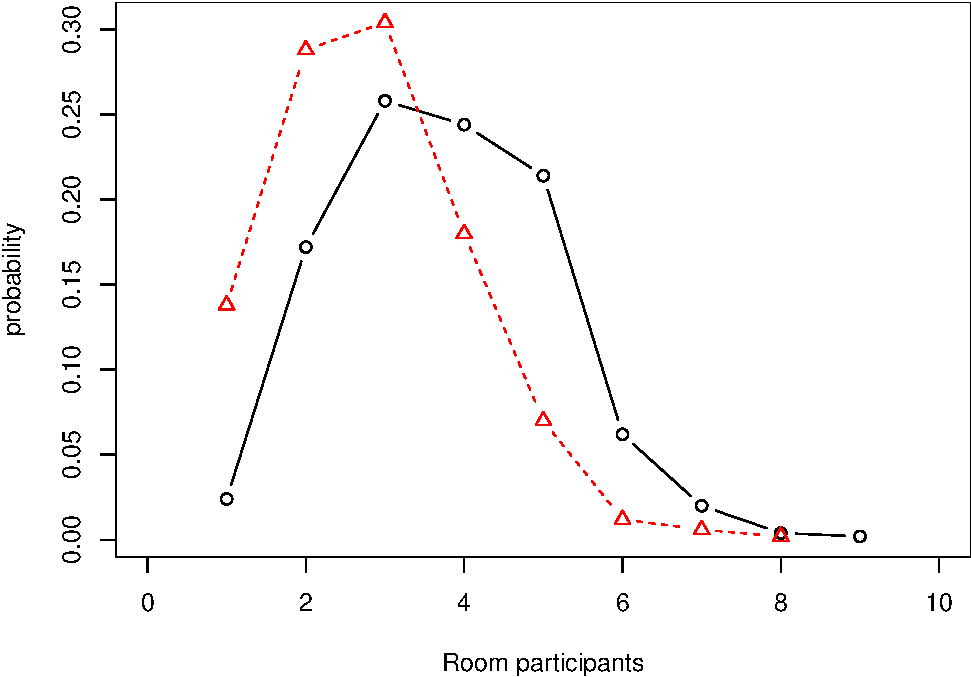
\includegraphics{Figures/unnamed-chunk-11-1.pdf}

\begin{Shaded}
\begin{Highlighting}[]
\CommentTok{# Add winner dots}

\NormalTok{winners <-}\StringTok{ }\ControlFlowTok{function}\NormalTok{() \{}
\NormalTok{    out <-}\StringTok{ }\KeywordTok{matrix}\NormalTok{(}\DataTypeTok{ncol =} \DecValTok{2}\NormalTok{, }\DataTypeTok{nrow =} \DecValTok{3}\NormalTok{)}
    \KeywordTok{rownames}\NormalTok{(out) <-}\StringTok{ }\KeywordTok{levels}\NormalTok{(treatment)}
    \KeywordTok{colnames}\NormalTok{(out) <-}\StringTok{ }\KeywordTok{c}\NormalTok{(}\StringTok{"hour"}\NormalTok{, }\StringTok{"final"}\NormalTok{)}
\NormalTok{    w <-}\StringTok{ }\KeywordTok{head}\NormalTok{(}\KeywordTok{which}\NormalTok{(final }\OperatorTok{>}\StringTok{ }\NormalTok{target }\OperatorTok{&}\StringTok{ }\NormalTok{treatment }\OperatorTok{==}\StringTok{ "race"}\NormalTok{), }\DecValTok{1}\NormalTok{)}
\NormalTok{    out[}\DecValTok{1}\NormalTok{, ] <-}\StringTok{ }\KeywordTok{c}\NormalTok{(hours[w], final[w])}
\NormalTok{    final.max <-}\StringTok{ }\KeywordTok{tapply}\NormalTok{(final, treatment, }\DataTypeTok{FUN =}\NormalTok{ max, }\DataTypeTok{na.rm =} \OtherTok{TRUE}\NormalTok{)}
\NormalTok{    w <-}\StringTok{ }\KeywordTok{which}\NormalTok{(final }\OperatorTok{==}\StringTok{ }\NormalTok{final.max[}\StringTok{"tournament"}\NormalTok{])}
\NormalTok{    out[}\DecValTok{2}\NormalTok{, ] <-}\StringTok{ }\KeywordTok{c}\NormalTok{(hours[w], final[w])}
\NormalTok{    w <-}\StringTok{ }\KeywordTok{which}\NormalTok{(final }\OperatorTok{==}\StringTok{ }\NormalTok{final.max[}\StringTok{"reserve"}\NormalTok{])}
\NormalTok{    out[}\DecValTok{3}\NormalTok{, ] <-}\StringTok{ }\KeywordTok{c}\NormalTok{(hours[w], final[w])}
\NormalTok{    out}
\NormalTok{\}}
\CommentTok{# points(winners())}

\CommentTok{# By treatment}
\NormalTok{x <-}\StringTok{ }\KeywordTok{aggregate}\NormalTok{(provisional.cap }\OperatorTok{~}\StringTok{ }\KeywordTok{round}\NormalTok{(hours) }\OperatorTok{+}\StringTok{ }\NormalTok{treatment, }\DataTypeTok{FUN =}\NormalTok{ mean)}
\NormalTok{index <-}\StringTok{ }\KeywordTok{split}\NormalTok{(}\DecValTok{1}\OperatorTok{:}\KeywordTok{nrow}\NormalTok{(x), x[, }\DecValTok{2}\NormalTok{])}
\KeywordTok{par}\NormalTok{(}\DataTypeTok{mfrow =} \KeywordTok{c}\NormalTok{(}\DecValTok{1}\NormalTok{, }\DecValTok{3}\NormalTok{))}
\ControlFlowTok{for}\NormalTok{ (i }\ControlFlowTok{in} \DecValTok{1}\OperatorTok{:}\DecValTok{3}\NormalTok{) \{}
    \KeywordTok{plot}\NormalTok{(x[index[[i]], }\OperatorTok{-}\DecValTok{2}\NormalTok{], }\DataTypeTok{ylim =} \KeywordTok{range}\NormalTok{(x[, }\DecValTok{3}\NormalTok{]), }\DataTypeTok{type =} \StringTok{"l"}\NormalTok{, }
        \DataTypeTok{lwd =} \DecValTok{2}\NormalTok{, }\DataTypeTok{col =} \KeywordTok{gray}\NormalTok{(}\FloatTok{0.85}\NormalTok{))}
    \KeywordTok{title}\NormalTok{(}\KeywordTok{names}\NormalTok{(index)[i])}
    \KeywordTok{abline}\NormalTok{(}\DataTypeTok{h =}\NormalTok{ target, }\DataTypeTok{lty =} \DecValTok{2}\NormalTok{, }\DataTypeTok{col =} \DecValTok{2}\NormalTok{)}
\NormalTok{\}}
\end{Highlighting}
\end{Shaded}

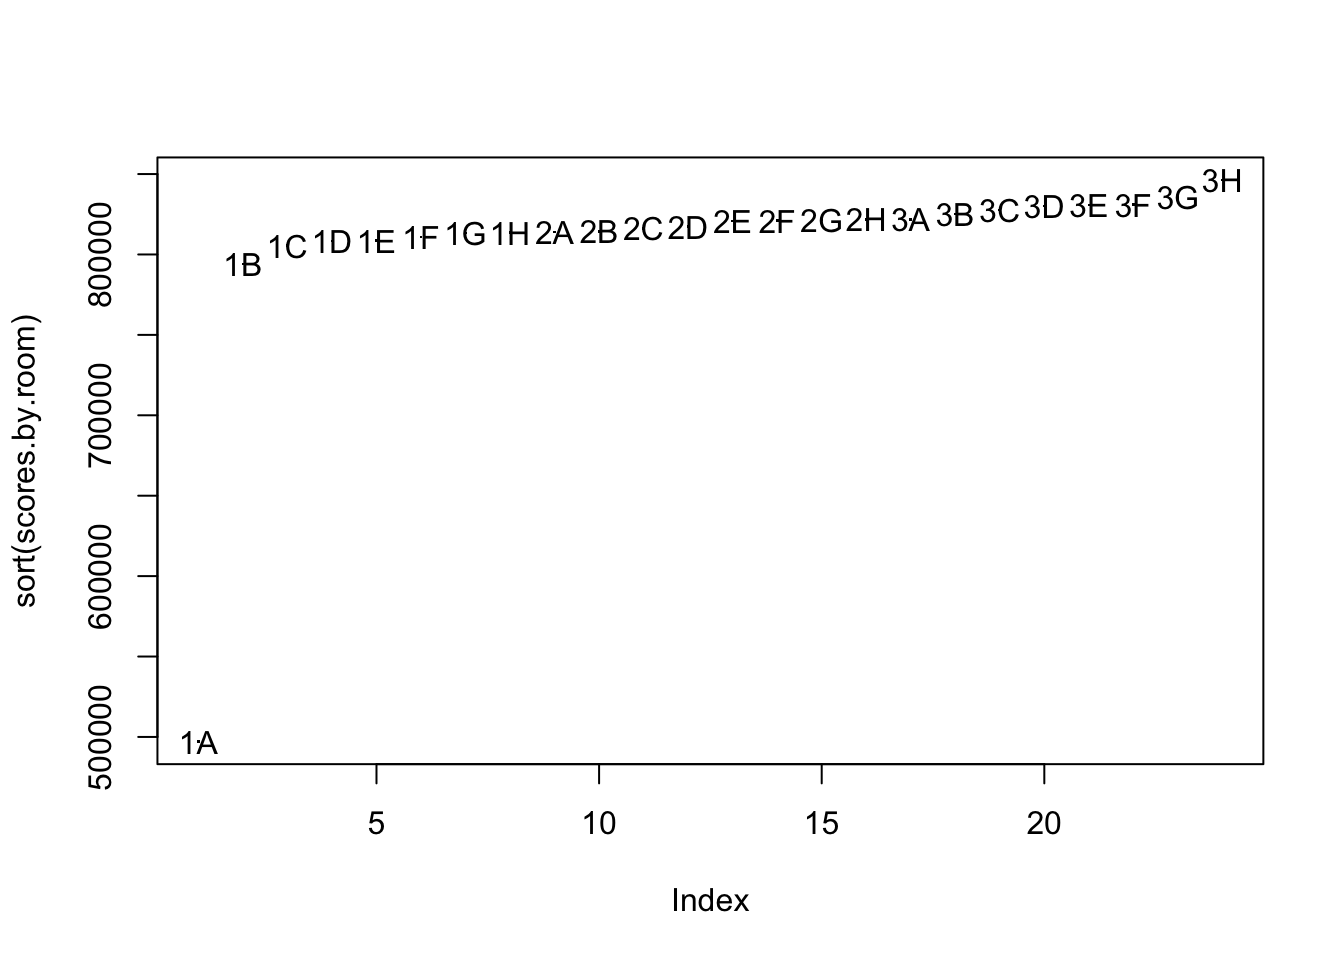
\includegraphics{Figures/unnamed-chunk-11-2.pdf}

\begin{Shaded}
\begin{Highlighting}[]
\CommentTok{# plot(aggregate(provisional.cap ~ round(hours), FUN=mean),}
\CommentTok{# type='l', lwd=2, col=gray(.85))}
\CommentTok{# points(aggregate(provisional ~ round(hours), FUN=mean))}


\CommentTok{# By treatment}
\NormalTok{i <-}\StringTok{ }\KeywordTok{split}\NormalTok{(}\DecValTok{1}\OperatorTok{:}\KeywordTok{nrow}\NormalTok{(dat), treatment)}
\NormalTok{xlim <-}\StringTok{ }\KeywordTok{range}\NormalTok{(timestamp)}
\NormalTok{ylim <-}\StringTok{ }\KeywordTok{range}\NormalTok{(provisional.cap)}

\NormalTok{max.score <-}\StringTok{ }\ControlFlowTok{function}\NormalTok{(x) \{}
\NormalTok{    n <-}\StringTok{ }\KeywordTok{length}\NormalTok{(x)}
\NormalTok{    y <-}\StringTok{ }\KeywordTok{numeric}\NormalTok{(n)}
    \ControlFlowTok{for}\NormalTok{ (i }\ControlFlowTok{in} \DecValTok{1}\OperatorTok{:}\NormalTok{n) y[i] <-}\StringTok{ }\KeywordTok{max}\NormalTok{(x[}\DecValTok{1}\OperatorTok{:}\NormalTok{i])}
    \KeywordTok{return}\NormalTok{(y)}
\NormalTok{\}}


\NormalTok{plot.scores <-}\StringTok{ }\ControlFlowTok{function}\NormalTok{(index, }\DataTypeTok{add =} \OtherTok{FALSE}\NormalTok{, ...) \{}
\NormalTok{    x <-}\StringTok{ }\NormalTok{timestamp[index]}
\NormalTok{    y <-}\StringTok{ }\NormalTok{provisional.cap[index]}
    \ControlFlowTok{if}\NormalTok{ (add }\OperatorTok{==}\StringTok{ }\OtherTok{FALSE}\NormalTok{) }
        \KeywordTok{plot}\NormalTok{(}\OtherTok{NA}\NormalTok{, }\OtherTok{NA}\NormalTok{, }\DataTypeTok{xlim =}\NormalTok{ xlim, }\DataTypeTok{ylim =}\NormalTok{ ylim)}
    \KeywordTok{points}\NormalTok{(x, y, }\DataTypeTok{pch =} \StringTok{"-"}\NormalTok{, ...)}
    \KeywordTok{abline}\NormalTok{(}\DataTypeTok{h =}\NormalTok{ target, }\DataTypeTok{lty =} \DecValTok{2}\NormalTok{, }\DataTypeTok{col =} \DecValTok{2}\NormalTok{)}
    \KeywordTok{lines}\NormalTok{(}\KeywordTok{smooth.spline}\NormalTok{(x, y, }\DataTypeTok{df =} \DecValTok{4}\NormalTok{))}
    \KeywordTok{abline}\NormalTok{(}\KeywordTok{lm}\NormalTok{(y }\OperatorTok{~}\StringTok{ }\NormalTok{x))}
    \KeywordTok{lines}\NormalTok{(x, }\KeywordTok{max.score}\NormalTok{(y))}
\NormalTok{\}}

\KeywordTok{par}\NormalTok{(}\DataTypeTok{mfrow =} \KeywordTok{c}\NormalTok{(}\DecValTok{1}\NormalTok{, }\DecValTok{3}\NormalTok{))}
\ControlFlowTok{for}\NormalTok{ (k }\ControlFlowTok{in} \KeywordTok{levels}\NormalTok{(treatment)) \{}
    \KeywordTok{plot.scores}\NormalTok{(i[[k]])}
    \KeywordTok{title}\NormalTok{(k)}
\NormalTok{\}}
\end{Highlighting}
\end{Shaded}

\includegraphics{Figures/unnamed-chunk-11-3.pdf}

\begin{Shaded}
\begin{Highlighting}[]
\CommentTok{# submission.cap <- ifelse(submission>15, 15, submission)}
\CommentTok{# boxplot(provisional/1e6 ~ submission.cap, pch='-')}
\CommentTok{# abline(h=0.8, col=2)}

\CommentTok{# Time series}
\NormalTok{l <-}\StringTok{ }\KeywordTok{split}\NormalTok{(dat, }\KeywordTok{paste}\NormalTok{(treatment, room))}
\NormalTok{xlim <-}\StringTok{ }\KeywordTok{range}\NormalTok{(timestamp)}
\NormalTok{ylim <-}\StringTok{ }\KeywordTok{c}\NormalTok{(}\FloatTok{0.7}\NormalTok{, }\FloatTok{0.9}\NormalTok{)}
\KeywordTok{par}\NormalTok{(}\DataTypeTok{mfrow =} \KeywordTok{c}\NormalTok{(}\DecValTok{5}\NormalTok{, }\DecValTok{5}\NormalTok{), }\DataTypeTok{mar =} \KeywordTok{c}\NormalTok{(}\DecValTok{2}\NormalTok{, }\DecValTok{2}\NormalTok{, }\DecValTok{1}\NormalTok{, }\DecValTok{1}\NormalTok{))}
\KeywordTok{sapply}\NormalTok{(l, }\ControlFlowTok{function}\NormalTok{(x) }\KeywordTok{plot}\NormalTok{(x}\OperatorTok{$}\NormalTok{timestamp, x}\OperatorTok{$}\NormalTok{provisional}\OperatorTok{/}\FloatTok{1e+06}\NormalTok{, }
    \DataTypeTok{xlim =}\NormalTok{ xlim, }\DataTypeTok{ylim =}\NormalTok{ ylim, }\DataTypeTok{pch =} \DecValTok{16}\NormalTok{))}
\end{Highlighting}
\end{Shaded}

\begin{verbatim}
## $`race 1`
## NULL
## 
## $`race 2`
## NULL
## 
## $`race 3`
## NULL
## 
## $`race 4`
## NULL
## 
## $`race 5`
## NULL
## 
## $`race 6`
## NULL
## 
## $`race 7`
## NULL
## 
## $`race 8`
## NULL
## 
## $`reserve 1`
## NULL
## 
## $`reserve 2`
## NULL
## 
## $`reserve 3`
## NULL
## 
## $`reserve 4`
## NULL
## 
## $`reserve 5`
## NULL
## 
## $`reserve 6`
## NULL
## 
## $`reserve 7`
## NULL
## 
## $`reserve 8`
## NULL
## 
## $`tournament 1`
## NULL
## 
## $`tournament 2`
## NULL
## 
## $`tournament 3`
## NULL
## 
## $`tournament 4`
## NULL
## 
## $`tournament 5`
## NULL
## 
## $`tournament 6`
## NULL
## 
## $`tournament 7`
## NULL
## 
## $`tournament 8`
## NULL
\end{verbatim}

\includegraphics{Figures/unnamed-chunk-11-4.pdf}

\section{Identification}\label{identification}

\newcommand\target{}
\newcommand\deadline{}

\subsection{The model}\label{the-model}

For each room \((l=1, ..., L)\), we observe the count of participants
\(y_l\) among the \(n_l\) registered competitors who have been assigned
to some treatment \(w_l\in\{0, 1, 2\}\). The count of participating
competitors is the realization of a random variable \(Y_l\) that depends
on a vector of room characteristics \(z_l=(x_l, w_l)\) that include the
assignment \(w_l\) and additional room characteristics \(x_l\). We
assume that \(Y_l\) is distributed as a binomial variable with
parameters \(n_l\) and \(p(x_l, \theta)\) where \(p(x, \theta)\)
describes the probability for a competitor to participate in a room
described by the vector \(x\). The model is then the following:

\begin{equation}
    \label{model}
    Y_{l} \sim \text{Binomial}(N_l, p(x_l, \theta)) \quad \text{for each } l=1,...,L.
\end{equation}

In binomial linear models, the probability function \(p(x, \theta)\) is
related to a linear prediction through a one-to-one transformation
called the link function (see xxxx). Following our theoretical approach,
participation is one for those with abilities above a given value:

\[
    Y_{l} = 1 \iff  \text{ability}  \geq m_{l}
\]

where \(m_l\) is the marginal type for the room. Given \(F_l(\cdot)\)
the distribution of individual abilities in each room, the probability
of entry is:

\begin{equation} 
    p(m_l, \theta) = 1 - F_l(m_l)
\end{equation}

The marginal type is determined by the zero profit condition:

\begin{equation}
    \label{zero profit}
    R_l(m_l) = m_l^\alpha y_0^\beta t_0^\gamma
\end{equation}

where the \(R_l(m_l)\) is the expected revenue of the marginal type in a
given room and it must be equal to the costs evaluated at the deadline
\(t_0\) and the target \(y_0\).

If we assume one single prize \(q=1\) (and we normalize the cost of
meeting the deadline to one \(t_0^\gamma=1\)) the zero profit condition
becomes:

\begin{equation}
    F_l(m_l)^{n_l-1} = m_l^\alpha y_0^\beta 
\end{equation}

By raising to the power \(1/(n_l-1)\) both sides of the equation, we
obtain a structural relationship between the probability of entry (eq.
XXX) and the marginal type, the number of registered competitors, and
the cost function.

\[
    p(x_l, \theta) = 1 - \left[m_l^\alpha y_0^\beta \right]^{1/(n_l-1)} \qquad \text{with } \alpha\leq-1, \beta\geq1.
\]

As a result, one could use a ``method of moments'' to estimate the
parameters \(\theta=(\alpha, \beta, m_l)\) (\(y_0\) and \(n_l\) are
observed).

\subsection{Estimation}\label{estimation}

First, we rewrite the probability \(p(x, \theta)\) in the following way:

\[
    p(x_l, \theta) = 1 - \theta_1 x_l^{\theta_2}
\]

where we denote the (observed) target by \(x_l\) and the vector of
parameters by \(\theta=(\theta_1, \theta_2)\) where
\(\theta_1 \equiv m_l^{\alpha/(n_l-1)}\) and
\(\theta_2 \equiv \beta/(n_l-1)\). Assume that \(n_l=n\) for each
\(l=1,...,L\).

Let \(Y_1, Y_2, ..., Y_L\) be the count of participants generated by our
binomial-distribution model. The likelihood is:

\[
    \mathcal{L} = \prod_{l=1}^L \binom{n_l}{y_l} p(x_l, \theta)^{y_l} [1-p(x_l, \theta)]^{n_l - y_l}
\]

The log-likelihood is:

\[
        ll = \sum_{l=1}^L  y_l\log(p(x_l, \theta)) + (n_l - y_l) \log(1-p(x_l, \theta))
\]

where we omit the binomial coefficient as it is a constant that does not
affect estimation.

Using our model into the aboev eqution:

\[
    ll = \sum_{l=1}^L  y_l\log(1 - \theta_1 x_l^{\theta_2})
         + (n - y_l) [\log(\theta_1) +  \theta_2\log(x_l)]
\]

Let the summation be denoted by \(\sum y_l = \bar y\). We can rewrite
the ll expression:

\[
    ll = (L n - \bar y)\log(\theta_1) +  \sum_{l=1}^L  y_l\log(1 - \theta_1 x_l^{\theta_2})
         +  (n - y_l) \theta_2\log(x_l)
\]

First order conditions are:

\[
    \frac{\partial  ll}{\partial \theta_1} 
    =  \frac{(L n - \bar y)}{\theta_1}  
        - \sum_{l=1}^L y_l \frac{x_l^{\theta_2}}{1 - \theta_1 x_l^{\theta_2}} = 0
    \]

\[
    \frac{\partial  ll}{\partial \theta_2} 
    =  \sum_{l=1}^L \left[- y_l \frac{x_l^{\theta_2}\theta_1 \log(x_l)}{1 - \theta_1 x_l^{\theta_2}} 
        + (n - y_l) \log(x_l) \right]= 0. 
\]

Try with simulations

\begin{Shaded}
\begin{Highlighting}[]
\NormalTok{n <-}\StringTok{ }\DecValTok{10}
\NormalTok{nsize <-}\StringTok{ }\DecValTok{199}
\NormalTok{theta1 <-}\StringTok{ }\FloatTok{0.75}
\NormalTok{theta2 <-}\StringTok{ }\FloatTok{0.05}
\NormalTok{params <-}\StringTok{ }\KeywordTok{c}\NormalTok{(theta1, theta2)}
\NormalTok{x <-}\StringTok{ }\KeywordTok{runif}\NormalTok{(nsize)}
\NormalTok{p <-}\StringTok{ }\DecValTok{1} \OperatorTok{-}\StringTok{ }\NormalTok{theta1 }\OperatorTok{*}\StringTok{ }\NormalTok{x}\OperatorTok{^}\NormalTok{theta2}
\CommentTok{# hist(prob, 100)}

\NormalTok{loglik <-}\StringTok{ }\ControlFlowTok{function}\NormalTok{(theta, data) \{}
\NormalTok{    theta1 <-}\StringTok{ }\NormalTok{theta[}\DecValTok{1}\NormalTok{]}
\NormalTok{    theta2 <-}\StringTok{ }\NormalTok{theta[}\DecValTok{2}\NormalTok{]}
\NormalTok{    x <-}\StringTok{ }\NormalTok{data}\OperatorTok{$}\NormalTok{x}
\NormalTok{    y <-}\StringTok{ }\NormalTok{data}\OperatorTok{$}\NormalTok{y}
\NormalTok{    n <-}\StringTok{ }\NormalTok{data}\OperatorTok{$}\NormalTok{n}
\NormalTok{    p <-}\StringTok{ }\DecValTok{1} \OperatorTok{-}\StringTok{ }\NormalTok{theta1 }\OperatorTok{*}\StringTok{ }\NormalTok{x}\OperatorTok{^}\NormalTok{theta2}
\NormalTok{    out <-}\StringTok{ }\KeywordTok{dbinom}\NormalTok{(y, n, p, }\DataTypeTok{log =}\NormalTok{ T)}
    \KeywordTok{return}\NormalTok{(}\OperatorTok{-}\KeywordTok{sum}\NormalTok{(out))}
\NormalTok{\}}

\CommentTok{# Simulate data}
\NormalTok{y <-}\StringTok{ }\KeywordTok{rbinom}\NormalTok{(nsize, }\DataTypeTok{size =}\NormalTok{ n, }\DataTypeTok{prob =}\NormalTok{ p)}

\CommentTok{# Example: loglik(c(0.5, 0.9), data.frame(y, x, n))}

\CommentTok{# MLE estimation}
\NormalTok{dat <-}\StringTok{ }\KeywordTok{data.frame}\NormalTok{(y, x, n)}
\NormalTok{theta.start <-}\StringTok{ }\KeywordTok{runif}\NormalTok{(}\DecValTok{2}\NormalTok{)}
\NormalTok{mle.est <-}\StringTok{ }\KeywordTok{optim}\NormalTok{(theta.start, loglik, }\DataTypeTok{data =}\NormalTok{ dat)}
\NormalTok{thetahat <-}\StringTok{ }\NormalTok{mle.est}\OperatorTok{$}\NormalTok{par}

\CommentTok{# Replications}
\NormalTok{out <-}\StringTok{ }\KeywordTok{replicate}\NormalTok{(}\DecValTok{1000}\NormalTok{, \{}
\NormalTok{    y <-}\StringTok{ }\KeywordTok{rbinom}\NormalTok{(nsize, }\DataTypeTok{size =}\NormalTok{ n, }\DataTypeTok{prob =}\NormalTok{ p)}
\NormalTok{    dat <-}\StringTok{ }\KeywordTok{data.frame}\NormalTok{(y, x, n)}
\NormalTok{    mle.est <-}\StringTok{ }\KeywordTok{optim}\NormalTok{(theta.start, loglik, }\DataTypeTok{data =}\NormalTok{ dat)}\OperatorTok{$}\NormalTok{par}
\NormalTok{\})}
\KeywordTok{boxplot}\NormalTok{(}\KeywordTok{t}\NormalTok{(out))}
\KeywordTok{abline}\NormalTok{(}\DataTypeTok{h =}\NormalTok{ params, }\DataTypeTok{col =} \DecValTok{2}\NormalTok{)}
\end{Highlighting}
\end{Shaded}

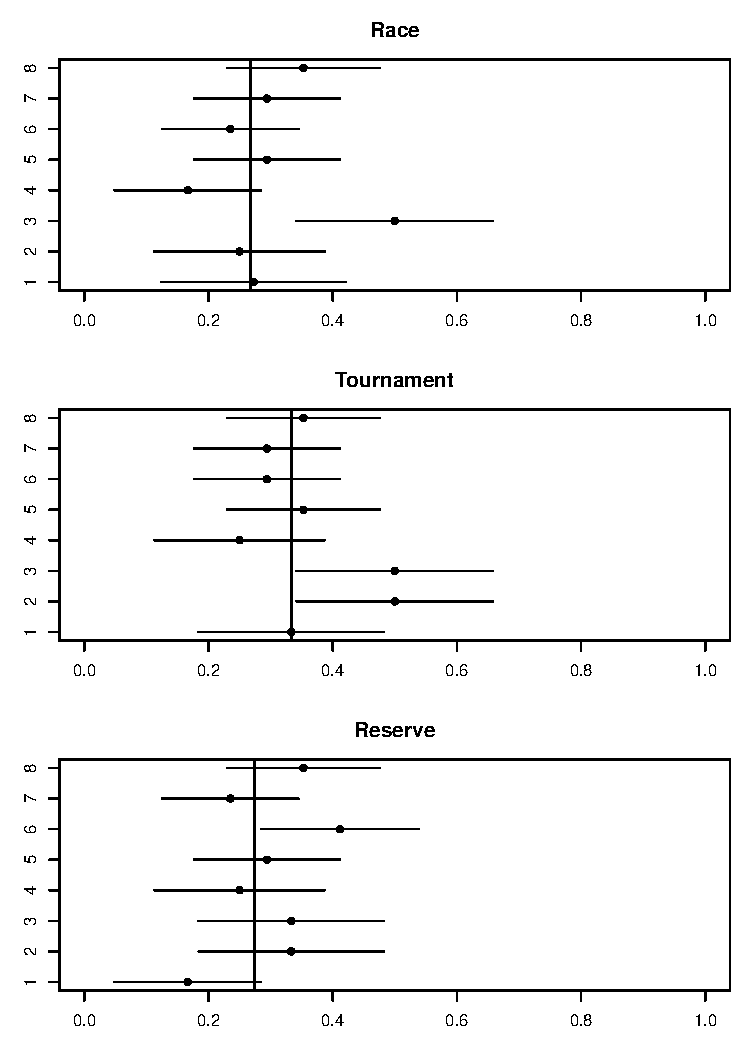
\includegraphics{Figures/unnamed-chunk-12-1.pdf}

\begin{Shaded}
\begin{Highlighting}[]
\NormalTok{truth <-}\StringTok{ }\ControlFlowTok{function}\NormalTok{(x) }\DecValTok{1} \OperatorTok{-}\StringTok{ }\NormalTok{params[}\DecValTok{1}\NormalTok{] }\OperatorTok{*}\StringTok{ }\NormalTok{x}\OperatorTok{^}\NormalTok{params[}\DecValTok{2}\NormalTok{]}

\CommentTok{# Now I can 'predictions' on what would happen with different}
\CommentTok{# 'x' distribution}
\NormalTok{prediction <-}\StringTok{ }\ControlFlowTok{function}\NormalTok{(x) }\DecValTok{1} \OperatorTok{-}\StringTok{ }\NormalTok{thetahat[}\DecValTok{1}\NormalTok{] }\OperatorTok{*}\StringTok{ }\NormalTok{x}\OperatorTok{^}\NormalTok{thetahat[}\DecValTok{2}\NormalTok{]}

\CommentTok{# Compare with logistic regression}
\NormalTok{N <-}\StringTok{ }\KeywordTok{rep}\NormalTok{(n, nsize)}
\NormalTok{logistic <-}\StringTok{ }\KeywordTok{glm}\NormalTok{(}\KeywordTok{cbind}\NormalTok{(y, N) }\OperatorTok{~}\StringTok{ }\NormalTok{x, }\DataTypeTok{family =} \KeywordTok{binomial}\NormalTok{(logit))}
\NormalTok{prediction.logistic <-}\StringTok{ }\ControlFlowTok{function}\NormalTok{(x) \{}
\NormalTok{    yhat <-}\StringTok{ }\KeywordTok{coef}\NormalTok{(logistic)[}\DecValTok{1}\NormalTok{] }\OperatorTok{+}\StringTok{ }\KeywordTok{coef}\NormalTok{(logistic)[}\DecValTok{2}\NormalTok{] }\OperatorTok{*}\StringTok{ }\NormalTok{x}
    \KeywordTok{exp}\NormalTok{(yhat)}\OperatorTok{/}\NormalTok{(}\DecValTok{1} \OperatorTok{+}\StringTok{ }\KeywordTok{exp}\NormalTok{(yhat))}
\NormalTok{\}}

\CommentTok{# FIGURE}
\KeywordTok{curve}\NormalTok{(truth, }\DataTypeTok{xlab =} \StringTok{"Room covariate"}\NormalTok{, }\DataTypeTok{ylim =} \KeywordTok{c}\NormalTok{(}\DecValTok{0}\NormalTok{, }\DecValTok{1}\NormalTok{))}
\KeywordTok{curve}\NormalTok{(prediction, }\DataTypeTok{add =} \OtherTok{TRUE}\NormalTok{, }\DataTypeTok{lty =} \DecValTok{2}\NormalTok{)}
\KeywordTok{curve}\NormalTok{(}\KeywordTok{prediction.logistic}\NormalTok{(x), }\DataTypeTok{add =} \OtherTok{TRUE}\NormalTok{, }\DataTypeTok{lty =} \DecValTok{3}\NormalTok{)}
\KeywordTok{legend}\NormalTok{(}\StringTok{"topright"}\NormalTok{, }\KeywordTok{c}\NormalTok{(}\StringTok{"Truth"}\NormalTok{, }\StringTok{"Estimated"}\NormalTok{, }\StringTok{"Logistic"}\NormalTok{), }\DataTypeTok{lty =} \DecValTok{1}\OperatorTok{:}\DecValTok{3}\NormalTok{)}
\end{Highlighting}
\end{Shaded}

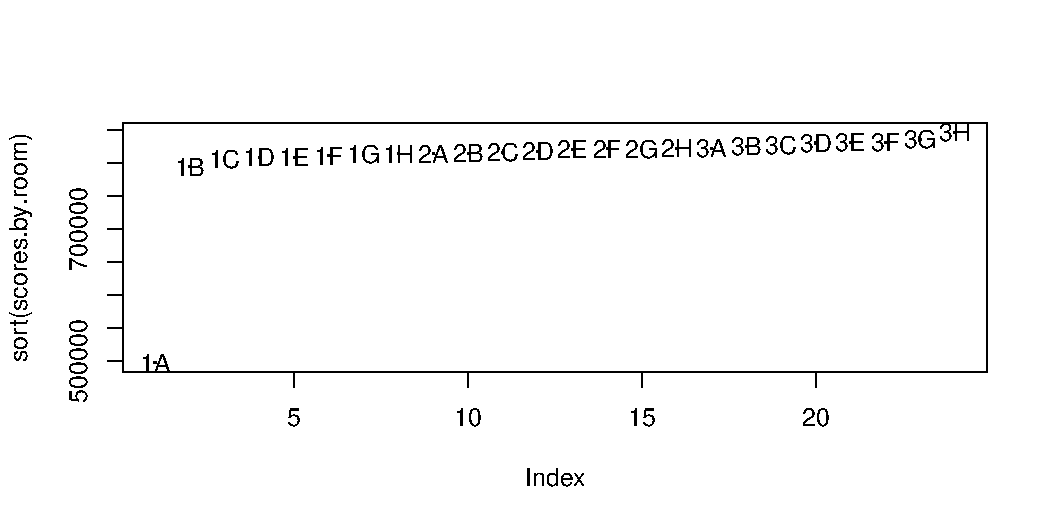
\includegraphics{Figures/unnamed-chunk-12-2.pdf}

\section{Identification (old)}\label{identification-old}

\subsection{Example with the Uniform
distribution}\label{example-with-the-uniform-distribution}

Imagine that the distribution \(F_\theta\) is uniform on \((0, \theta)\)
and the cost ability \(c_a(x) = 1/x\). Then the zero profit condition
\eqref{zero profit} becomes

\begin{align}
    \left(\frac{m}{\theta}\right)^{n-1} m = \beta x_l 
\end{align}

Solving for the marginal type gives:

\begin{align}
    m = \left(\beta x_l  \theta^{n-1}\right)^{1/n}
\end{align}

So, the probability of participation \eqref{probability} becomes

\begin{align}
    p(x_l, \theta) 
        & = 1 - F_\theta(m) \\
        & = 1 - \frac{\left(\beta x_l \theta^{n-1}\right)^{1/n} }{\theta} \\
        & = 1 - \left(\frac{\beta x_l}{\theta}\right)^{1/n}.
\end{align}

Because it is non-linear in its parameters, the model is not
identifiable {[}need proof{]}. However, we can re-parametrize the model
with \(\beta/\theta \equiv \eta\) to make the parameter \(\eta\)
identifiable.

\begin{figure}
\centering
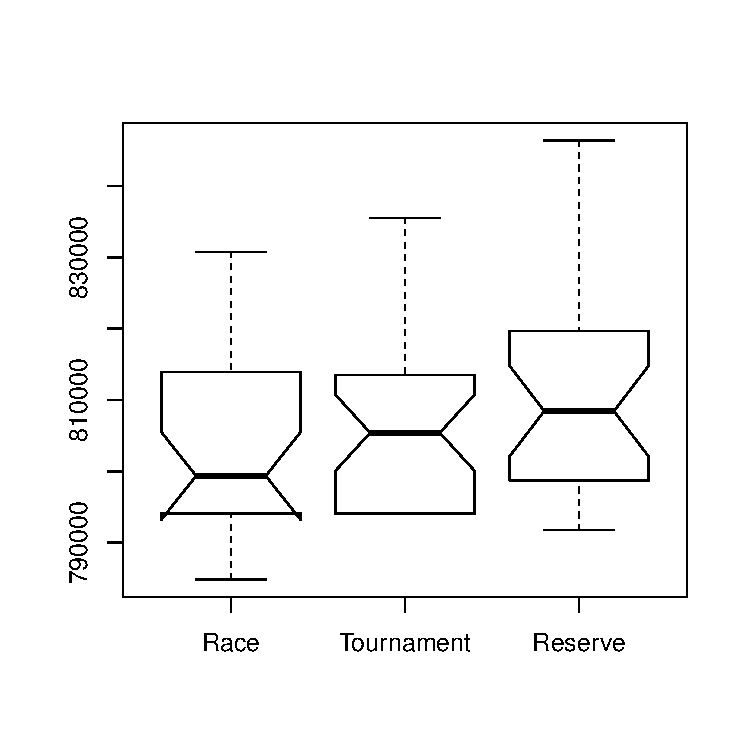
\includegraphics{Figures/unnamed-chunk-13-1.pdf}
\caption{Simulated distribution of participants with uniform
distribution. Parameters are \(\eta=0.1\) and \(n=15\). Data simulated
500 times. Dashed curve had higher costs (\(x_l=1.5\)) than the solid
curve (\(x_l=0.5\)).}
\end{figure}

\subsection{Example with Beta
distribution}\label{example-with-beta-distribution}

In this example, we assume abilities are drawn from a lognormal
distribution with parameters \(\mu\) and \(\sigma\).

\subsection{Estimation}\label{estimation-1}

Our aim is to estimate the parameters \(\theta\) and \(\beta\) and to
evaluate whether costs are different between the three competition modes
under study: race, tournament, tournament + requirement.

It is natural to estimate the parameters \(\theta\) by maximum
likelihood because the ability distribution (and therefore the
distribution of the outcomes) is known. The estimation criterion used
here is the maximization of the \emph{deviance}.

The deviance is:

\begin{equation}
    D(\theta) = -2 \sum Y \log (\frac{N p(x, \theta)}{Y}) 
        + (N - Y) \log ( \frac{N - N p}{N - Y}).
\end{equation}

Note that the deviance is a function of the likelihood (see xxx pg.
xxx).

\begin{Shaded}
\begin{Highlighting}[]
\CommentTok{# Define likelihood}
\NormalTok{structreg <-}\StringTok{ }\ControlFlowTok{function}\NormalTok{(x, y, }\DataTypeTok{wt =} \KeywordTok{rep}\NormalTok{(}\DecValTok{1}\NormalTok{, }\KeywordTok{length}\NormalTok{(y)), }\DataTypeTok{intercept =} \OtherTok{TRUE}\NormalTok{, }
    \DataTypeTok{start =} \KeywordTok{rep}\NormalTok{(}\DecValTok{0}\NormalTok{, p), ...) \{}
\NormalTok{    fmin <-}\StringTok{ }\ControlFlowTok{function}\NormalTok{(beta, X, y, w) \{}
\NormalTok{        p <-}\StringTok{ }\DecValTok{1} \OperatorTok{-}\StringTok{ }\NormalTok{(beta }\OperatorTok\StringTok{ }\NormalTok{X)}\OperatorTok{^}\NormalTok{(}\DecValTok{1}\OperatorTok{/}\NormalTok{n)  }\CommentTok{# Function of parameters}
        \OperatorTok{-}\KeywordTok{sum}\NormalTok{(}\DecValTok{2} \OperatorTok{*}\StringTok{ }\NormalTok{w }\OperatorTok{*}\StringTok{ }\KeywordTok{ifelse}\NormalTok{(y, }\KeywordTok{log}\NormalTok{(p), }\KeywordTok{log}\NormalTok{(}\DecValTok{1} \OperatorTok{-}\StringTok{ }\NormalTok{p)))}
\NormalTok{    \}}
    \CommentTok{# gmin <- function(beta, X, y, w) \{ # Gradient here!  \}}
    \ControlFlowTok{if}\NormalTok{ (}\KeywordTok{is.null}\NormalTok{(}\KeywordTok{dim}\NormalTok{(x))) }
        \KeywordTok{dim}\NormalTok{(x) <-}\StringTok{ }\KeywordTok{c}\NormalTok{(}\KeywordTok{length}\NormalTok{(x), }\DecValTok{1}\NormalTok{)}
\NormalTok{    dn <-}\StringTok{ }\KeywordTok{dimnames}\NormalTok{(x)[[}\DecValTok{2}\NormalTok{]]}
    \ControlFlowTok{if}\NormalTok{ (}\OperatorTok{!}\KeywordTok{length}\NormalTok{(dn)) }
\NormalTok{        dn <-}\StringTok{ }\KeywordTok{paste}\NormalTok{(}\StringTok{"Var"}\NormalTok{, }\DecValTok{1}\OperatorTok{:}\KeywordTok{ncol}\NormalTok{(x), }\DataTypeTok{sep =} \StringTok{""}\NormalTok{)}
\NormalTok{    p <-}\StringTok{ }\KeywordTok{ncol}\NormalTok{(x) }\OperatorTok{+}\StringTok{ }\NormalTok{intercept}
    \ControlFlowTok{if}\NormalTok{ (intercept) \{}
\NormalTok{        x <-}\StringTok{ }\KeywordTok{cbind}\NormalTok{(}\DecValTok{1}\NormalTok{, x)}
\NormalTok{        dn <-}\StringTok{ }\KeywordTok{c}\NormalTok{(}\StringTok{"(Intercept)"}\NormalTok{, dn)}
\NormalTok{    \}}
    \ControlFlowTok{if}\NormalTok{ (}\KeywordTok{is.factor}\NormalTok{(y)) }
\NormalTok{        y <-}\StringTok{ }\NormalTok{(}\KeywordTok{unclass}\NormalTok{(y) }\OperatorTok{!=}\StringTok{ }\DecValTok{1}\NormalTok{)}
    \CommentTok{# fit <- optim(start, fmin, gmin, X = x, y = y, w = wt,}
    \CommentTok{# method = 'BFGS', ...)}
\NormalTok{    fit <-}\StringTok{ }\KeywordTok{optim}\NormalTok{(}\FloatTok{0.5}\NormalTok{, fmin, }\DataTypeTok{X =}\NormalTok{ x, }\DataTypeTok{y =}\NormalTok{ y, }\DataTypeTok{w =}\NormalTok{ wt, }\DataTypeTok{method =} \StringTok{"BFGS"}\NormalTok{, }
\NormalTok{        ...)}
    \KeywordTok{names}\NormalTok{(fit}\OperatorTok{$}\NormalTok{par) <-}\StringTok{ }\NormalTok{dn}
    \KeywordTok{cat}\NormalTok{(}\StringTok{"}\CharTok{\textbackslash{}n}\StringTok{Coefficients:}\CharTok{\textbackslash{}n}\StringTok{"}\NormalTok{)}
    \KeywordTok{print}\NormalTok{(fit}\OperatorTok{$}\NormalTok{par)}
    \KeywordTok{cat}\NormalTok{(}\StringTok{"}\CharTok{\textbackslash{}n}\StringTok{Residual Deviance:"}\NormalTok{, }\KeywordTok{format}\NormalTok{(fit}\OperatorTok{$}\NormalTok{value), }\StringTok{"}\CharTok{\textbackslash{}n}\StringTok{"}\NormalTok{)}
    \KeywordTok{cat}\NormalTok{(}\StringTok{"}\CharTok{\textbackslash{}n}\StringTok{Convergence message:"}\NormalTok{, fit}\OperatorTok{$}\NormalTok{convergence, }\StringTok{"}\CharTok{\textbackslash{}n}\StringTok{"}\NormalTok{)}
    \KeywordTok{invisible}\NormalTok{(fit)}
\NormalTok{\}}

\CommentTok{# Create data}
\NormalTok{ilogit <-}\StringTok{ }\ControlFlowTok{function}\NormalTok{(x) }\KeywordTok{exp}\NormalTok{(x)}\OperatorTok{/}\NormalTok{(}\DecValTok{1} \OperatorTok{+}\StringTok{ }\KeywordTok{exp}\NormalTok{(x))}
\NormalTok{n <-}\StringTok{ }\DecValTok{50000}
\NormalTok{competitors <-}\StringTok{ }\DecValTok{5}
\NormalTok{x1 <-}\StringTok{ }\KeywordTok{rchisq}\NormalTok{(competitors, }\DataTypeTok{df =} \DecValTok{3}\NormalTok{)}
\NormalTok{x2 <-}\StringTok{ }\KeywordTok{runif}\NormalTok{(n)}
\NormalTok{x3 <-}\StringTok{ }\KeywordTok{rnorm}\NormalTok{(n)}
\NormalTok{X <-}\StringTok{ }\KeywordTok{cbind}\NormalTok{(}\KeywordTok{rep}\NormalTok{(}\DecValTok{1}\NormalTok{, }\KeywordTok{length}\NormalTok{(x1)), x1, x2, x3)}
\NormalTok{betas <-}\StringTok{ }\KeywordTok{c}\NormalTok{(}\OperatorTok{-}\FloatTok{2.5}\NormalTok{, }\FloatTok{0.1}\NormalTok{, }\FloatTok{0.25}\NormalTok{, }\FloatTok{0.5}\NormalTok{)}
\NormalTok{fc <-}\StringTok{ }\KeywordTok{ilogit}\NormalTok{(X }\OperatorTok\StringTok{ }\NormalTok{betas)  ## This the fixed cost}
\NormalTok{p <-}\StringTok{ }\DecValTok{1} \OperatorTok{-}\StringTok{ }\NormalTok{fc}\OperatorTok{^}\NormalTok{(}\DecValTok{1}\OperatorTok{/}\NormalTok{competitors)}
\NormalTok{y <-}\StringTok{ }\KeywordTok{rbinom}\NormalTok{(}\DataTypeTok{n =}\NormalTok{ n, }\DataTypeTok{size =}\NormalTok{ competitors, }\DataTypeTok{prob =}\NormalTok{ p)}

\CommentTok{# Objective function}
\NormalTok{fmin <-}\StringTok{ }\ControlFlowTok{function}\NormalTok{(beta, X, y, w, competitors) \{}
\NormalTok{    p <-}\StringTok{ }\DecValTok{1} \OperatorTok{-}\StringTok{ }\KeywordTok{ilogit}\NormalTok{(X }\OperatorTok\StringTok{ }\NormalTok{beta)}\OperatorTok{^}\NormalTok{(}\DecValTok{1}\OperatorTok{/}\NormalTok{competitors)  }\CommentTok{# Function of parameters}
    \OperatorTok{-}\KeywordTok{sum}\NormalTok{(}\DecValTok{2} \OperatorTok{*}\StringTok{ }\NormalTok{w }\OperatorTok{*}\StringTok{ }\KeywordTok{ifelse}\NormalTok{(y, }\KeywordTok{log}\NormalTok{(p), }\KeywordTok{log}\NormalTok{(}\DecValTok{1} \OperatorTok{-}\StringTok{ }\NormalTok{p)))}
\NormalTok{\}}

\NormalTok{b.start <-}\StringTok{ }\KeywordTok{runif}\NormalTok{(}\KeywordTok{length}\NormalTok{(betas))}
\NormalTok{(out <-}\StringTok{ }\KeywordTok{optim}\NormalTok{(b.start, fmin, }\DataTypeTok{X =}\NormalTok{ X, }\DataTypeTok{y =}\NormalTok{ y, }\DataTypeTok{competitors =}\NormalTok{ competitors, }
    \DataTypeTok{w =} \KeywordTok{rep}\NormalTok{(}\DecValTok{1}\NormalTok{, }\KeywordTok{length}\NormalTok{(y)))}\OperatorTok{$}\NormalTok{par)}
\end{Highlighting}
\end{Shaded}

\begin{verbatim}
## [1] -12.8289579   0.3957879   1.3857148   2.0384539
\end{verbatim}

\begin{Shaded}
\begin{Highlighting}[]
\KeywordTok{rbind}\NormalTok{(out}\OperatorTok{/}\NormalTok{competitors, betas)}
\end{Highlighting}
\end{Shaded}

\begin{verbatim}
##            [,1]       [,2]     [,3]      [,4]
##       -2.565792 0.07915759 0.277143 0.4076908
## betas -2.500000 0.10000000 0.250000 0.5000000
\end{verbatim}

\subsection{More examples}\label{more-examples}

Suppose F is lognormal(\(\mu, \sigma\)), then the zero profit condition
is:

\begin{align}
    \left[\frac 12 +\frac 12 \left(\frac{\log{m}-\mu}{\sqrt{2\sigma}}\right)\right] = a^{-1/(n-1)} K_l
\end{align}

\begin{verbatim}
# xxx
zeroprofit <- function(x, mu, sigma, n) {
    x * plnorm(x, meanlog=mu, sdlog=sigma)^(n-1)
}
for (i in 3:10)
    curve(zeroprofit(x, i, 10, 10), add=TRUE, lty=i)
\end{verbatim}

\begin{Shaded}
\begin{Highlighting}[]
\CommentTok{# Clear}
\KeywordTok{rm}\NormalTok{(}\DataTypeTok{list =} \KeywordTok{ls}\NormalTok{())}

\CommentTok{# Libraries}
\KeywordTok{require}\NormalTok{(xtable)}
\KeywordTok{require}\NormalTok{(moments)}
\KeywordTok{require}\NormalTok{(races)}

\CommentTok{# Data}
\KeywordTok{data}\NormalTok{(races)}
\KeywordTok{attach}\NormalTok{(races)}

\CommentTok{# TABLE 1.}
\NormalTok{size <-}\StringTok{ }\KeywordTok{ave}\NormalTok{(submit, }\KeywordTok{paste}\NormalTok{(treatment, room), }\DataTypeTok{FUN =}\NormalTok{ length)}
\NormalTok{(m <-}\StringTok{ }\KeywordTok{aggregate}\NormalTok{(submit }\OperatorTok{~}\StringTok{ }\NormalTok{room }\OperatorTok{+}\StringTok{ }\NormalTok{size }\OperatorTok{+}\StringTok{ }\NormalTok{treatment, }\DataTypeTok{FUN =}\NormalTok{ sum))}
\end{Highlighting}
\end{Shaded}

\begin{verbatim}
##    room size  treatment submit
## 1     1    9       race      2
## 2     2   10       race      2
## 3     3   10       race      5
## 4     4   10       race      1
## 5     5   15       race      4
## 6     6   15       race      3
## 7     7   15       race      4
## 8     8   15       race      5
## 9     1   10 tournament      3
## 10    2   10 tournament      5
## 11    3   10 tournament      5
## 12    4   10 tournament      2
## 13    5   15 tournament      5
## 14    6   15 tournament      4
## 15    7   15 tournament      4
## 16    8   15 tournament      5
## 17    1   10    reserve      1
## 18    2   10    reserve      3
## 19    3   10    reserve      3
## 20    4   10    reserve      2
## 21    5   15    reserve      4
## 22    6   15    reserve      6
## 23    7   15    reserve      3
## 24    8   15    reserve      5
\end{verbatim}


\end{document}